% !TEX root = main.tex
% !TEX program = pdflatex
\pdfminorversion=7
\documentclass[final,5p,times,number]{elsarticle}

\usepackage{amsmath,amssymb,amsfonts}
\usepackage[ruled,vlined,linesnumbered]{algorithm2e}
\usepackage{textcomp}
\usepackage{xcolor}
\usepackage{booktabs}
\usepackage{listings}
\usepackage{url}
\usepackage{multirow}
\usepackage{tabularx}
\usepackage{lmodern}
\usepackage[final]{microtype}
\usepackage{tikz}
\usetikzlibrary{arrows.meta,positioning,fit,calc}
\graphicspath{{./}}
\emergencystretch=2em
\setlength{\textfloatsep}{5pt plus 1pt minus 2pt}
\setlength{\floatsep}{5pt plus 1pt minus 2pt}
\setlength{\intextsep}{5pt plus 1pt minus 2pt}
\setlength{\dbltextfloatsep}{5pt plus 1pt minus 2pt}
\setlength{\dblfloatsep}{5pt plus 1pt minus 2pt}
\setlength{\abovecaptionskip}{2pt}
\setlength{\belowcaptionskip}{0pt}
\makeatletter
\setlength{\@fptop}{0pt}
\setlength{\@fpsep}{5pt plus 1pt minus 2pt}
\setlength{\@fpbot}{0pt plus 1fil}
\long\def\@makecaption#1#2{%
  \vskip\abovecaptionskip
  \sbox\@tempboxa{\footnotesize #1. #2}%
  \ifdim \wd\@tempboxa >\hsize
    \footnotesize #1. #2\par
  \else
    \global \@minipagefalse
    \hb@xt@\hsize{\hfil\box\@tempboxa\hfil}%
  \fi
  \vskip\belowcaptionskip}
\makeatother
\usepackage[hidelinks]{hyperref}
\hypersetup{
  pdfborder={0 0 0},
  colorlinks=false
}
\newcommand{\figref}[1]{\hyperref[#1]{Fig.~\ref*{#1}}}
\newcommand{\figureref}[1]{\hyperref[#1]{Figure~\ref*{#1}}}
\newcommand{\figsref}[2]{\hyperref[#1]{Figs.~\ref*{#1}} and~\hyperref[#2]{\ref*{#2}}}

\biboptions{sort&compress}

\journal{Computers \& Security}

\begin{document}

\begin{frontmatter}

\title{LoopFuzz: \textcolor{blue}{Feedback-Driven Orchestration} for LLM-Guided Stateful Fuzzing of Response-Visible Protocols}

\author[inst1]{Ketang Chen}
\ead{3250006913@student.must.edu.mo}
\author[inst1]{Xiaolei Ren\corref{cor1}}
\ead{xlren@must.edu.mo}
\cortext[cor1]{Corresponding author: Xiaolei Ren. Email address: xlren@must.edu.mo}

\affiliation[inst1]{organization={Macau University of Science and Technology},
            addressline={Avenida Wai Long, Taipa},
            city={Macau},
            country={China}}

\begin{abstract}
Stateful protocol fuzzing is difficult because syntactically valid messages generated by large language models (LLMs) can still violate the live session state. \textcolor{blue}{LoopFuzz uses runtime-evidence-guided orchestration for textual or semi-textual request-response protocols: request candidates pass parseability, response acceptability, state-reachability, and gain checks before queue promotion, while scheduling actions remain bounded hints. Across nine AFLNet/ChatAFL-lineage targets, the integrated condition correlates with statistically supported IPSM-edge gains (BH-adjusted, $n=10$) on eight targets versus AFLNet and six versus the controlled ChatAFL-lineage baseline, with additional positive trends requiring larger samples; branch endpoints are supported on seven and four targets. Forked-daapd remains a boundary case, preliminary triage is not a vulnerability-yield ranking, and NSFuzz, Mosquitto, and MBFuzzer rows are diagnostic. Because the archive lacks a \emph{LoopFuzz-no-admission} arm and candidate-level admission logs, these results are integrated-policy evidence, not a causal estimate of the $P/U/R/G$ gate.}
\end{abstract}

\begin{keyword}
Protocol fuzzing \sep Large language models \sep \textcolor{blue}{Feedback-driven orchestration} \sep Stateful testing \sep Counterexample-guided local repair
\end{keyword}

\end{frontmatter}
\small

\section{Introduction}
Network protocol implementations remain difficult security targets because correctness depends on interaction history rather than isolated inputs~\cite{aflnet,stateafl,sgf_usenix22,formatted_stateful_greybox_fuzzing_2024,resolverfuzz_query_response_2024}. A File Transfer Protocol (FTP) server, for example, rejects a well-formed \texttt{PASS} command if no valid \texttt{USER} command has established the login state. Unlike file fuzzing, protocol fuzzing must preserve message syntax, temporal order, and request-response progress across a multi-step session~\cite{resolverfuzz_query_response_2024,mbfuzzer_mqtt_2025,bleem_packet_sequence_2023,logos_log_guided_fuzzing_2024,diane_identifying_fuzzing_triggers_2021,corecrisis_context_aware_2025}.

Traditional coverage-guided fuzzers work well for stateless parsers. They fit network servers poorly when later behavior depends on earlier valid exchanges~\cite{directed_greybox_fuzzing_2017,seed_selection_successful_fuzzing_2021,one_fuzzing_strategy_rule_2022,regression_greybox_fuzzing_2021,efficient_errors_2022}. Stateful greybox fuzzers such as AFLNet and StateAFL partially close this gap. They infer progress from responses and replay valid traces~\cite{aflnet,stateafl,sgf_usenix22,profuzzbench_benchmark_stateful_protocol_2021,snapfuzz_high_throughput_fuzzing_2022,bleem_packet_sequence_2023,formatted_stateful_greybox_fuzzing_2024}. Even so, byte-level mutation still struggles to synthesize the context-sensitive messages needed to cross deep protocol boundaries.

Large language models (LLMs) offer a plausible source of such messages. ChatAFL and later LLM-assisted fuzzers show that a model can extract structure from specifications, logs, or documentation and produce fluent candidates~\cite{chatafl,fuzz4all_universal_fuzzing_large_2024,llmif_augmented_large_language_2024,matter_llm_specification_2024,carpetfuzz_documentation_2023,prompt_fuzzing_fuzz_driver_2024,large_language_models_are_2023,large_language_models_are_2024}. But fluency is not enough. A request can be grammatically plausible and still be invalid for the live session state. Such executions spend budget without improving queue quality.

LoopFuzz places a runtime admission controller between LLM generation and queue admission. It treats the LLM as a hypothesis generator rather than an oracle: hypotheses are derived from Request for Comments (RFC) fragments, seed traces, and observed responses; failed executions become counterexamples for local repair; and inferred protocol state machine (IPSM) feedback steers frontier scheduling and plateau-triggered assistance. \textcolor{blue}{The name \emph{LoopFuzz} emphasizes runtime feedback over LLM proposals and local repair, not control-theoretic stability, formal verification of protocol semantics, model behavior, or server correctness.}

The scope is deliberately narrower than universal protocol fuzzing. LoopFuzz is designed and evaluated for textual or semi-textual request-response protocols where candidate parseability can be checked locally and response-derived progress is visible to the fuzzer. Binary, encrypted, or tightly formatted protocols such as Transport Layer Security (TLS), Datagram Transport Layer Security (DTLS), QUIC, Secure Shell (SSH), Internet Protocol Security (IPsec), and similar targets would require dedicated adapters for message construction, rejection classification, and state extraction before the same control policy could be evaluated. We do not claim that the current evidence validates LoopFuzz on those protocol families.

The methodological contributions of this paper are as follows:
\begin{itemize}
    \item \textbf{Hypothesis-Driven Modeling.} LoopFuzz derives message grammars and field constraints from RFC fragments, seed traces, and observed responses, and maintains them as explicit, auditable runtime hypotheses.
    \item \textbf{Runtime-Evidence Boundary.} LoopFuzz inserts a runtime-evidence boundary between the LLM and the durable queue. It checks structure before trial execution and uses bounded execution evidence to evaluate response acceptability, state reachability, and downstream gain before durable queue promotion.
    \item \textbf{Counterexample-Guided Local Repair.} LoopFuzz preserves failed request-response traces as counterexamples and exposes a prompt-constrained, audit-logged local repair path; in this evaluation, we treat repair as an auditable control mechanism rather than an independently quantified source of endpoint gains or a hard single-patch guarantee.
    \item \textbf{State-Aware Scheduling.} LoopFuzz leverages IPSM topology, state productivity, and adaptive plateau detection to prioritize underexplored frontier states and to request model assistance only when mutation alone stalls.
\end{itemize}

\textcolor{blue}{Accordingly, the paper evaluates LoopFuzz as an integrated campaign-control policy. Here, a ChatAFL comparator means the controlled ChatAFL-lineage baseline\footnote{\textcolor{blue}{Not the original artifact; Table~\ref{tab:chatafl_config_scope} lists model, temperature, token-cap, and control-logic changes.}} in Table~\ref{tab:chatafl_config_scope}. The archive associates LoopFuzz with higher state exploration and branch coverage on most primary targets, but does not isolate $P/U/R/G$ from token budget, temperature, scheduling, repair, or plateau activation; external artifacts remain diagnostic.}

\section{Background and Motivation}

\begin{table*}[ht]
\centering
\caption{Representative fuzzer taxonomy}
\label{tab:taxonomy}
\renewcommand{\arraystretch}{1.3}
\footnotesize
\setlength{\tabcolsep}{3pt}
\resizebox{\textwidth}{!}{%
\begin{tabular}{l l c c l}
\toprule
\textbf{System} & \textbf{Input prior} & \textbf{State signal} & \textbf{Admission rule} & \textbf{Online repair} \\
\midrule
Coverage-guided mutation fuzzing~\cite{directed_greybox_fuzzing_2017,seed_selection_successful_fuzzing_2021}         & Byte mutation & None & None & No \\
AFLNet~\cite{aflnet}              & Packet capture (PCAP) mutation  & Response & Novelty & No \\
StateAFL~\cite{stateafl}          & PCAP mutation  & Memory & Novelty & No \\
ChatAFL~\cite{chatafl}            & Context-guided LLM generation & Interaction history & No runtime admission boundary & No \\
\textbf{LoopFuzz (ours)}         & \textbf{LLM hypotheses} & \textcolor{blue}{\textbf{AFLNet-style IPSM (same as AFLNet) + frontier scheduling}} & \textbf{Runtime admission} & \textbf{Yes} \\
\bottomrule
\end{tabular}}
\normalsize
\end{table*}

Table~\ref{tab:taxonomy} contrasts LoopFuzz with representative fuzzers. ChatAFL-style systems use protocol and interaction context to guide LLM generation. LoopFuzz studies a stricter campaign-control setting in which generated proposals are mediated by runtime evidence before they influence a long-running stateful campaign. The evaluation measures this setting as an integrated strategy rather than as an isolated test of the admission boundary alone.

\subsection{Coverage-Guided Fuzzing vs. Network Targets}
A coverage-guided fuzzer operates through a repeated feedback cycle of seed selection, mutation, execution, coverage measurement, and novelty-based queue update~\cite{seed_selection_successful_fuzzing_2021,one_fuzzing_strategy_rule_2022,regression_greybox_fuzzing_2021,efficient_errors_2022}.
This loop is effective for file parsers, but network targets impose three constraints that matter here:
\begin{enumerate}
    \item \textbf{Temporal state dependence:} server behavior depends on the order and semantics of earlier messages, not only on the current payload~\cite{aflnet,stateafl,sgf_usenix22,formatted_stateful_greybox_fuzzing_2024}.
    \item \textbf{Strict message format:} protocols require delimiters, field layouts, and often checksum or length consistency, so many mutated messages die before they reach deeper logic~\cite{gramatron_effective_grammar_aware_2021,griffin_grammar_free_dbms_2022,formatted_stateful_greybox_fuzzing_2024}.
    \item \textbf{Execution instability:} sockets, forking daemons, and asynchronous response handling complicate both coverage collection and campaign throughput~\cite{snapfuzz_high_throughput_fuzzing_2022}.
\end{enumerate}

\subsection{Stateful Greybox Fuzzing (SGF)}
SGF addresses this gap by treating the target through an IPSM. In the AFLNet lineage, this machine is an approximate response-derived graph, not a deterministic model of the protocol semantics. We use the lightweight abstraction $\mathcal{M}=(Q,\widehat{\Delta},q_0)$ to describe the scheduling signal, where:
\begin{itemize}
    \item $Q$ denotes the set of response-derived state identifiers;
    \item $\widehat{\Delta}\subseteq Q\times Q$ denotes the observed transition relation induced by concrete executions; and
    \item $q_0$ denotes the initial connection state.
\end{itemize}

AFLNet-style fuzzers infer $Q$ and $\widehat{\Delta}$ from observed responses and use that structure to bias later exploration. Response codes, response texts, and adapter summaries create state identifiers and error hints; they are not modeled as a separate output function here. The abstraction can be partial and history-dependent because asynchronous replies, races, timeouts, daemon state, and environment can make the same sequence expose different response evidence. LoopFuzz therefore uses the IPSM as a scheduling and progress signal, not as a complete protocol semantics model.

\subsection{LLM Integration into Protocol Fuzzing}
LLMs make it easier to propose structure-aware protocol messages from RFC text, interaction history, or observed responses. That helps with syntax and message diversity, but it does not solve the harder control problem: a fluent request can still be wrong for the live session state.

\subsection{A Motivating Example: Semantic Drift}

\begin{figure}[t!]
\centering
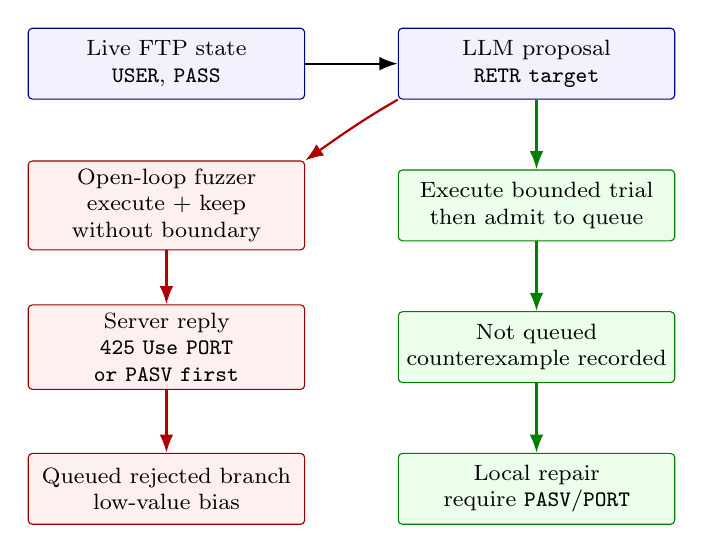
\begin{tikzpicture}[
    font=\footnotesize,
    >=Latex,
    box/.style={draw, rounded corners=1.5pt, align=center, minimum height=9mm, text width=33mm, fill=white, inner sep=3pt},
    open/.style={box, fill=red!6, draw=red!60!black},
    closed/.style={box, fill=green!8, draw=green!50!black},
    neutral/.style={box, fill=blue!5, draw=blue!55!black},
    arrow/.style={->, thick}
]
\node[neutral] (state) at (0,3.0) {Live FTP state\\\texttt{USER}, \texttt{PASS}};
\node[neutral] (llm) at (4.7,3.0) {LLM proposal\\\texttt{RETR target}};
\node[open] (openadmit) at (0,1.2) {Open-loop fuzzer\\execute + keep\\without boundary};
\node[open] (reject) at (0,-0.6) {Server reply\\\texttt{425 Use PORT}\\\texttt{or PASV first}};
\node[open] (waste) at (0,-2.4) {Queued rejected branch\\low-value bias};
\node[closed] (gate) at (4.7,1.2) {Execute bounded trial\\then admit to queue};
\node[closed] (cex) at (4.7,-0.6) {Not queued\\counterexample recorded};
\node[closed] (repair) at (4.7,-2.4) {Local repair\\require \texttt{PASV}/\texttt{PORT}};
\draw[arrow] (state) -- (llm);
\draw[arrow, red!70!black] (llm.south west) to[out=210,in=35] (openadmit.north east);
\draw[arrow, red!70!black] (openadmit) -- (reject);
\draw[arrow, red!70!black] (reject) -- (waste);
\draw[arrow, green!50!black] (llm) -- (gate);
\draw[arrow, green!50!black] (gate) -- (cex);
\draw[arrow, green!50!black] (cex) -- (repair);
\end{tikzpicture}
\caption{Illustrative, non-archived FTP semantic-drift pattern with bounded post-trial admission and counterexample evidence}
\label{fig:motivation}
\end{figure}

Consider the FTP session in \figref{fig:motivation}. After \texttt{USER} and \texttt{PASS}, the LLM proposes \texttt{RETR target}; the request is syntactically fluent but premature because no \texttt{PASV} or \texttt{PORT} data channel exists. We call this failure \emph{semantic drift}: a locally plausible request violates the live session precondition. LoopFuzz handles it through runtime validation. The controller checks local structure, runs a bounded trial, treats the rejection response as negative evidence, avoids durable queue promotion, and can record the failed trace as counterexample evidence for a local \texttt{PASV}/\texttt{PORT} repair.

This example is illustrative rather than empirical trace evidence. \textcolor{blue}{The selected archives preserve run-level \texttt{fuzzer\_stats}, \texttt{plot\_data}, queue/IPSM artifacts, response files, and raw plateau replies, but not candidate-level joins for state, candidate, response, $P/U/R/G$, promotion, and repair. Semantic drift is therefore a motivation, not a measured prevalence: Table~\ref{tab:candidate_admission_gap} lacks $U$-fail/rejection rows, while Table~\ref{tab:bug_crash_triage} reports replayable protocol-oracle/logical artifacts that ground the admission boundary beyond \figref{fig:motivation}.}

\section{Related Work}
We position LoopFuzz against the prior lines that are closest in mechanism and evaluation.

Earlier structure-aware fuzzing used explicit structure, inferred snippets, token constraints, or grammar guidance to preserve validity~\cite{snipuzz_black_box_fuzzing_2021,token_level_fuzzing_2021,gramatron_effective_grammar_aware_2021,griffin_grammar_free_dbms_2022,no_grammar_no_problem_2023,likely_invariants_feedback_2021,mundofuzz_grammar_inference_2022}. These systems improve input quality, but they do not address the control problem that arises when an external model proposes state-dependent protocol messages.

Stateful greybox and state-aware network-service fuzzing address protocol interaction more directly. AFLNet, StateAFL, NSFuzz, and the broader SGF line infer or expose state structure from server responses, process memory, or program variables~\cite{aflnet,stateafl,nsfuzz,sgf_usenix22,profuzzbench_benchmark_stateful_protocol_2021}. They then use that structure to prioritize rare or productive traces. These systems define the broader comparison landscape, but they do not all expose the same state abstraction, instrumentation path, or archived endpoint metrics.

Later systems extend this idea to packet-sequence exploration, format-sensitive protocol fuzzing, and communication-heavy environments~\cite{bleem_packet_sequence_2023,formatted_stateful_greybox_fuzzing_2024,logos_log_guided_fuzzing_2024,msgfuzzer_message_sequence_guided_2024,resolverfuzz_query_response_2024,mbfuzzer_mqtt_2025,fuzzusb_hybrid_stateful_fuzzing_2022,dtls_fuzzer_dtls_protocol_2022,edhoc_fuzzer_edhoc_protocol_2023,tron_fuzzing_linux_network_2025}. LoopFuzz asks a narrower question: given an AFLNet-style response-derived IPSM and the ChatAFL-style LLM proposal path, does an integrated runtime-admission strategy make the campaign more reliable? \textcolor{blue}{AFLNet and the controlled ChatAFL-lineage baseline are therefore the closest implementation-lineage baselines in the primary experiment.} StateAFL, SGF, NSFuzz, Bleem, Logos, and MBFuzzer remain important external comparison points; their different state abstractions, instrumentation paths, and artifact semantics motivate the separate diagnostic tables in the evaluation.

Adjacent work studies state-aware or interaction-heavy fuzzing in robotic policies, firmware, Linux drivers, middleware, hardware, and embedded systems~\cite{pgfuzz_policy_guided_fuzzing_2021,android_smarttvs_vulnerability_discovery_2021,fuzzware_mmio_2022,statefuzz_linux_driver_2022,differential_fuzzing_data_distribution_2024,fuzzing_hardware_like_software_2022,coverage_guided_fuzzing_embedded_2023}. Although not all are protocol fuzzers, they reinforce the point that state feedback can dominate raw mutation quality.

Target-aware scheduling and semantic validation form another relevant line. Directed greybox fuzzing, seed selection, and strategy adaptation study how to steer budget toward high-value behaviors~\cite{directed_greybox_fuzzing_2017,windranger_blocks_2022,when_analysis_2025,seed_selection_successful_fuzzing_2021,one_fuzzing_strategy_rule_2022,regression_greybox_fuzzing_2021,efficient_errors_2022}. Semantic validation and fuzz-driver generation show that stronger inputs often require an explicit acceptance interface~\cite{one_engine_to_fuzz_em_all_2021,apicraft_fuzz_driver_2021}. LoopFuzz applies that lesson to LLM proposals.

Our repair loop also borrows the broad counterexample-driven intuition from counterexample-guided abstraction refinement (CEGAR) in formal verification~\cite{cegar_cav2000}. The analogy is limited: LoopFuzz records failed executions as concrete evidence for local message-hypothesis patches, but it does not construct a formal abstraction, prove refinement soundness or completeness, or compute minimal counterexamples.

Work on dependency inference, data-flow guidance, and learned signals outside protocol fuzzing also supports treating guidance as bounded evidence rather than as an oracle~\cite{rulf_rust_library_fuzzing_2021,smartian_analyses_2021,magneto_step_wise_approach_2024}.

LLM guidance addresses the synthesis bottleneck more directly. ChatAFL performs context-guided LLM generation from RFCs and interaction histories~\cite{chatafl}; adjacent systems use LLMs for general input generation, documentation-guided constraints, device fuzzing, or fuzz-driver generation~\cite{fuzz4all_universal_fuzzing_large_2024,llmif_augmented_large_language_2024,docter_documentation_guided_fuzzing_2022,carpetfuzz_documentation_2023,matter_llm_specification_2024,prompt_fuzzing_fuzz_driver_2024}. Our work is closest to ChatAFL, and differs by adding an explicit runtime admission boundary: LoopFuzz asks whether a proposal should be admitted, whether its hypothesis survives runtime evidence, and how the IPSM should guide the next query.

Benchmarking practice is also part of the context. ProFuzzBench established a reusable baseline for repeated protocol-fuzzing experiments~\cite{profuzzbench_benchmark_stateful_protocol_2021}. Recent methodology work shows how easily comparisons become unstable without fixed budgets, repeated trials, and careful interpretation of coverage signals~\cite{sok_prudent_evaluation_practices_2024,reliability_benchmarking_2022,many_stack_2022}. We follow that guidance because runtime-validated assistance is especially sensitive to campaign history.

\section{LoopFuzz Design}

\figref{fig:arch} summarizes the three coupled loops in LoopFuzz: the Grammar Hypothesis Loop, the Fuzz Execution Loop, and the LLM Intervention Loop.

\begin{figure*}[t!]
\centering
\definecolor{lfblue}{RGB}{55,95,130}
\definecolor{lforange}{RGB}{178,108,35}
\definecolor{lfpurple}{RGB}{112,79,145}
\definecolor{lfgreen}{RGB}{67,128,93}
\definecolor{lfred}{RGB}{168,82,73}
\resizebox{\textwidth}{!}{%
\begin{tikzpicture}[
    font=\footnotesize,
    >=Latex,
    block/.style={draw, rounded corners=2pt, align=center, minimum height=9.2mm, text width=31mm, fill=white, inner xsep=3.2pt, inner ysep=3pt, line width=0.55pt},
    grammar/.style={block, draw=lfblue, fill=lfblue!7},
    fuzz/.style={block, draw=lforange, fill=lforange!8},
    llm/.style={block, draw=lfpurple, fill=lfpurple!7},
    gate/.style={block, draw=lfgreen, fill=lfgreen!9, text width=34mm, minimum height=10.5mm, line width=0.7pt},
    fail/.style={block, draw=lfred, fill=lfred!8},
    panel/.style={draw, rounded corners=4pt, line width=0.45pt},
    arrow/.style={->, line width=0.7pt, draw=black!68},
    feedback/.style={->, line width=0.7pt, dashed, draw=black!58},
    reject/.style={->, line width=0.7pt, draw=lfred!85!black},
    repairflow/.style={->, line width=0.75pt, dashed, draw=lfred!85!black},
    monitorline/.style={-, line width=0.7pt, dashed, draw=lfpurple!85!black},
    label/.style={font=\bfseries\footnotesize, align=center},
    legend/.style={font=\scriptsize, align=left}
]
\draw[panel, draw=lfblue!45, fill=lfblue!3] (-5.80,-2.12) rectangle (-1.00,5.24);
\draw[panel, draw=lforange!50, fill=lforange!4] (-0.56,-2.12) rectangle (4.24,5.24);
\draw[panel, draw=lfpurple!45, fill=lfpurple!4] (4.68,-2.12) rectangle (9.48,5.24);

\node[label, text=lfblue] at (-3.40,4.86) {Grammar Hypothesis Loop};
\node[label, text=lforange] at (1.84,4.86) {Fuzz Execution Loop};
\node[label, text=lfpurple] at (7.08,4.86) {LLM Intervention Loop};
\draw[draw=lfblue!20, line width=0.45pt] (-5.44,4.42) -- (-1.36,4.42);
\draw[draw=lforange!22, line width=0.45pt] (-0.20,4.42) -- (3.88,4.42);
\draw[draw=lfpurple!20, line width=0.45pt] (5.04,4.42) -- (9.12,4.42);

\node[grammar] (evidence) at (-3.40,3.58) {RFC fragments\\seed traces\\observed responses};
\node[grammar] (hyp) at (-3.40,2.06) {Message hypotheses\\grammar and\\constraints};
\node[grammar] (tier1) at (-3.40,0.54) {Tier-1 sampling\\parsed-region check\\{\scriptsize\textcolor{blue}{implemented; partial log}}};
\node[fail] (repair) at (-3.40,-1.24) {Tier-2 repair\\counterexample patch\\{\scriptsize\textcolor{blue}{implemented; partial log}}};

\node[fuzz, text width=35mm] (select) at (1.84,3.58) {State-aware\\seed selection};
\node[fuzz, text width=35mm] (exec) at (1.84,2.06) {Mutation and\\bounded execution};
\node[fuzz, text width=35mm] (update) at (1.84,0.54) {Coverage/IPSM\\update};
\node[gate, text width=44mm] (admit) at (1.84,-1.24) {Execute-then-admit\\$P$ before trial; $U/R/G$ after\\{\scriptsize\textcolor{blue}{implemented; no per-candidate log}}};

\node[llm] (plateau) at (7.08,3.58) {Periodic plateau\\monitor};
\node[llm] (prompt) at (7.08,2.06) {State prompt\\reuse guard};
\node[llm] (reply) at (7.08,0.54) {Structured reply\\schema validation};
\node[llm] (dispatch) at (7.08,-1.24) {Bounded action\\mutation, priority, redirection};

\draw[arrow, draw=lfblue!85!black] (evidence) -- (hyp);
\draw[arrow, draw=lfblue!85!black] (hyp) -- (tier1);
\draw[reject] (tier1.south) -- node[midway, font=\scriptsize, align=center,
  text=lfred!85!black, fill=lfblue!3, inner sep=1.1pt]
  {counterexample evidence accumulates} (repair.north);
\draw[reject] (repair.west) to[out=180,in=180,looseness=1.15] (hyp.west);

\draw[arrow, draw=lforange!85!black] (select) -- (exec);
\draw[arrow, draw=lforange!85!black] (exec) -- (update);
\draw[feedback, draw=lforange!85!black] (update.west) to[out=180,in=180,looseness=1.10] (select.west);

\draw[arrow, draw=lfpurple!85!black] (plateau) -- (prompt);
\draw[arrow, draw=lfpurple!85!black] (prompt) -- (reply);
\draw[arrow, draw=lfpurple!85!black] (reply) -- (dispatch);
\draw[monitorline] (update.east) -- ++(0.58,0) coordinate (monstem) |- (plateau.west);

\draw[arrow, draw=lfgreen!80!black] (dispatch.west) -- (admit.east);
\draw[arrow, draw=lfgreen!80!black, line width=1.0pt] (admit.north) -- (update.south);
\draw[repairflow] (admit.west) -- (repair.east);

\draw[monitorline] (-3.50,-2.55) -- (-2.70,-2.55);
\node[legend, anchor=west, text=black!70] at (-2.60,-2.55) {periodic edge-growth monitor};
\draw[repairflow] (1.45,-2.55) -- (2.25,-2.55);
\node[legend, anchor=west, text=lfred!85!black] at (2.35,-2.55) {not queued; recorded as counterexample};
\end{tikzpicture}}
\caption{LoopFuzz \textcolor{blue}{feedback-driven orchestration} architecture with bounded policy proposals, plateau-gated repair, and execute-then-admit request validation}
\label{fig:arch}
\end{figure*}

LoopFuzz preserves the stateful greybox fuzzing execution path while placing a control boundary between LLM output and durable queue admission. Request-producing outputs change the queue only after structural checks, bounded execution, and post-trial evidence support promotion. Non-request actions, such as target-state redirection or seed prioritization, remain schema-checked scheduling hints whose value is mediated by later AFLNet-style novelty logic. The four coupled components are grammar hypotheses, runtime admission, counterexample-guided repair, and state-aware scheduling.

\figureref{fig:arch} separates the method into three analytical feedback loops. The Grammar Hypothesis Loop builds and repairs message hypotheses from RFC knowledge, seed traces, and observed responses. The Fuzz Execution Loop performs state selection, mutation, bounded execution, IPSM update, and novelty checking. The LLM Intervention Loop is activated by a periodic plateau monitor, not by every execution, and returns either a validated continuation or a bounded control action.

\textcolor{blue}{The labels in \figref{fig:arch} are implemented control interfaces rather than a complete archived event ledger: hypothesis validation and Tier-2 repair are only partially logged, and candidate-level $P/U/R/G$ decisions are not archived (Tables~\ref{tab:candidate_admission_gap} and~\ref{tab:admission_accounting_archive}).} Tier-1 sampling accumulates evidence, Tier-2 repair uses counterexamples, schema validation checks replies, and bounded action dispatch maps a validated request proposal into a trial. Only request candidates that pass post-trial admission become durable queue entries; scheduling-only actions remain weaker hints.

\textcolor{blue}{\emph{Scope limitation.} Response-ambiguous DAAP/DACP-over-HTTP targets are boundary cases because status-code states do not normalize DAAP paths, session progress, or media-control phases.}

\subsection{Grammar Hypothesis Loop}
Let $\mathcal{L}(c, s, \Sigma)$ denote the LLM generation function under prompt context $c$, state summary $s$, and protocol knowledge $\Sigma$. LoopFuzz uses $\mathcal{L}$ in two stages: bounded initial enrichment preserves ChatAFL's template and seed path, while a lazily initialized hypothesis layer is activated at the first plateau event and then updated through sampled validation and local repair.

The Grammar Hypothesis Loop draws on three evidence sources when they are available: RFC fragments, queued seed traces or packet examples, and observed server responses, including response codes and error texts. For each message type $m$, the loop maintains a hypothesis $h_m=(G_m,\Phi_m)$. Here, $G_m$ is an Augmented Backus--Naur Form (ABNF)-style or template-style production, and $\Phi_m$ stores field constraints such as length bounds, enumerations, token dependencies, and simple cross-field relations. This representation is stricter than free-form text, lighter than a full specification, and cheap to validate online.

The evidence sources need not be complete. LoopFuzz requires testable hypotheses rather than a full formal protocol specification; runtime admission decides whether those hypotheses can affect the campaign. \textcolor{blue}{This lazy layer yields non-trivial updates only when response evidence exposes parseable grammar regions; low sampled pass rates in Table~\ref{tab:admission_accounting_archive} mark sparse or irregular traces where runs rely mainly on plateau scheduling and runtime admission.}

\subsection{Runtime Admission Controller}
The runtime admission controller makes queue-admission decisions for request-producing model outputs in two stages. Stage 1 checks structural well-formedness and local parseability before a proposal is sent. Stage 2 runs a bounded trial and evaluates the observed response, inferred state movement, and coverage or IPSM gain. A request candidate $x$ is retained only if
\[
A(x)=P(x) \land U(x) \land R(x) \land G(x),
\]
where $P$ denotes pre-trial parseability and $U$, $R$, and $G$ are post-trial predicates. $U$ captures response-grounded acceptability; $R$ requires a usable response-derived state sequence, target/frontier reachability, or escape from a rejection sink; and $G$ asks whether the trial adds coverage, unseen IPSM structure, or queue value relative to the pre-trial campaign state. If $P$ fails, the proposal is not executed. If any post-trial predicate fails, the trace may update counterexample or productivity evidence, but it is not promoted. Non-request control actions are outside this formula: they undergo schema and identifier checks, alter only scheduling metadata, and are evaluated indirectly by later executions.

\textcolor{blue}{Table~\ref{tab:admission_predicates} gives the operational definition and minimum fields needed to replay an admission decision; because normalized admission-event logs are absent, it is a controller specification and log schema, not a recovered causal-results table.}

\begin{table*}[!t]
\centering
\caption{Request-admission predicates and audit fields}
\label{tab:admission_predicates}
{\scriptsize
\setlength{\tabcolsep}{3.2pt}
\renewcommand{\arraystretch}{1.05}
\resizebox{\textwidth}{!}{%
\begin{tabular}{>{\raggedright\arraybackslash}p{0.07\textwidth}
                >{\raggedright\arraybackslash}p{0.18\textwidth}
                >{\raggedright\arraybackslash}p{0.25\textwidth}
                >{\raggedright\arraybackslash}p{0.22\textwidth}
                >{\raggedright\arraybackslash}p{0.20\textwidth}}
\toprule
\textbf{Pred.} & \textbf{Input} & \textbf{Pass} & \textbf{Fail} & \textbf{Log/effect} \\
\midrule
\textbf{$P$}\\Parse &
Pre: action/request, $h_m$. &
Schema; fields; bounds; delimiters; local parse. &
Malformed action; missing field/term.; type/len./parse err. &
Id, type, flags, err., hyp.; no exec. \\
\midrule
\textbf{$U$}\\Accept &
Post: resp., code/state, timeout/reset, adapter. &
Non-reject state seq.; or $h=1\!\rightarrow\!2$, $N_s\ge10$, $p_s\ge0.1$. &
4xx/5xx; timeout/reset/drop; no state seq.; unparsable. &
Extractor, code, timeout, $h,N,D,p$, reason, override; no promote. \\
\midrule
\textbf{$R$}\\Reach &
Post: src, state seq., target/frontier. &
\textcolor{blue}{Usable seq. that hits target/frontier or escapes sink.} &
\textcolor{blue}{Non-reject but no target/frontier movement; same sink; no seq.; unmapped state.} &
Src/dst, seq., target, escape, productivity; novelty deferred. \\
\midrule
\textbf{$G$}\\Gain &
Post: coverage, IPSM novelty, favored status. &
New coverage; new IPSM node/path/edge; favored entry. &
$U/R$ pass; no coverage/IPSM/queue gain. &
Bit/branch/IPSM deltas, favored, gain reason, promote flag; all-pass promotes. \\
\bottomrule
\end{tabular}}
}
\end{table*}

\textcolor{blue}{The conjunction is a staged specification, not a statistical-independence claim. The predicates are semantically separable by counterexample: an FTP \texttt{RETR} before \texttt{PASV}/\texttt{PORT} can pass $P$ yet fail $U$ with a live \texttt{425}; a syntactically valid request can receive a non-rejection response yet repeat the current non-target state, so $U$ passes but $R$ fails; and a candidate can reach the scheduled target/frontier state but only rediscover an existing transition with no branch delta or favored queue entry, so $R$ passes but $G$ fails. The archive lacks candidate-level joins to measure correlations among these predicates, so Table~\ref{tab:admission_predicates} should be read as an operational boundary rather than evidence that all predicates independently explain endpoint gains.}

\textcolor{blue}{A decisive \emph{LoopFuzz-no-admission} arm would keep the endpoint, prompts, 64 plateau calls, 4096 tokens, temperatures, IPSM scheduling, triggers, and schemas, but bypass $P/U/R/G$. It is absent, so current experiments test only the integrated policy.}

\subsubsection{Structured Output and Parseability}
The plateau stage accepts either a concrete next-request candidate or a bounded structured action. Runtime validation checks structural well-formedness, field types, length bounds, delimiters, terminators, and action-schema consistency, then tests local parseability against current message hypotheses. This can reject malformed interventions before trial execution; usefulness is decided only by the post-trial predicates in Table~\ref{tab:admission_predicates}.

\subsubsection{Response-Grounded Acceptability}
Parseability alone does not rule out semantic prematurity. LoopFuzz therefore classifies bounded-trial responses and treats a non-rejection response as positive evidence. For the primary text protocols, response-code priors cover the FTP, Simple Mail Transfer Protocol (SMTP), Real Time Streaming Protocol (RTSP), Hypertext Transfer Protocol (HTTP), Session Initiation Protocol (SIP), and Internet Printing Protocol (IPP) adapters: state ids are classified by $\lfloor s/100\rfloor$, and classes 4 and 5 initialize $h(s)=1$ as likely rejection. Forked-daapd uses the HTTP-style extractor because Digital Audio Access Protocol/Digital Audio Control Protocol (DAAP/DACP) requests are HTTP/1.1 requests with DAAP paths and query parameters. Timeouts, early disconnects, resets, and responses without a recoverable state sequence are negative execution evidence.

The earlier word ``rescue'' has a narrow implementation meaning. Protocol adapters map response bytes to state ids; they do not provide target-specific rescue thresholds. The only implemented rescue from a rejection prior is the uniform behavioral override in Table~\ref{tab:uniform_policies}: $h=1$ may become $h=2$ when $N_s\ge10$ and $p_s=D_s/(N_s+1)\ge0.1$. Conversely, $N_s\ge30$ and $p_s<0.005$ demotes initially unknown states for scheduling but is not a positive $U$ rescue. The controller therefore asks a narrow post-trial question: did live target behavior support promoting this candidate?

\begin{table*}[!t]
\centering
\caption{Protocol-adapter rules}
\label{tab:protocol_adapter_rules}
{\scriptsize
\setlength{\tabcolsep}{3.2pt}
\renewcommand{\arraystretch}{1.08}
\begin{tabularx}{\textwidth}{>{\raggedright\arraybackslash}p{0.18\textwidth}
>{\raggedright\arraybackslash}p{0.12\textwidth}
>{\raggedright\arraybackslash}X
>{\raggedright\arraybackslash}p{0.18\textwidth}}
\toprule
Targets & Opt. & State id & Reject prior \\
\midrule
LightFTP, bftpd, ProFTPD, Pure-FTPd &
\texttt{-P FTP} &
Line $\rightarrow$ 3-digit code; start 0. &
4xx/5xx $\rightarrow h=1$. \\
Exim &
\texttt{-P SMTP} &
Line $\rightarrow$ 3-digit code; start 0. &
4xx/5xx $\rightarrow h=1$. \\
Live555 &
\texttt{-P RTSP} &
\texttt{RTSP/} status $\rightarrow$ 3-digit code; others ignored. &
4xx/5xx $\rightarrow h=1$. \\
Kamailio &
\texttt{-P SIP} &
\texttt{SIP/} status $\rightarrow$ 3-digit code; others ignored. &
4xx/5xx $\rightarrow h=1$. \\
Forked-daapd &
\texttt{-P HTTP} &
HTTP status $\rightarrow$ 3-digit code; DAAP paths not states. &
4xx/5xx $\rightarrow h=1$. \\
Lighttpd1 &
\texttt{-P HTTP} &
HTTP status $\rightarrow$ 3-digit code; start 0. &
4xx/5xx $\rightarrow h=1$. \\
\bottomrule
\end{tabularx}
}
\end{table*}

\begin{table*}[!t]
\centering
\caption{Uniform policies}
\label{tab:uniform_policies}
{\scriptsize
\setlength{\tabcolsep}{3.2pt}
\renewcommand{\arraystretch}{1.08}
\begin{tabularx}{\textwidth}{>{\raggedright\arraybackslash}p{0.18\textwidth}
>{\raggedright\arraybackslash}p{0.12\textwidth}
>{\raggedright\arraybackslash}X
>{\raggedright\arraybackslash}p{0.18\textwidth}}
\toprule
Policy & Scope & Rule & Effect \\
\midrule
Timeout &
All targets &
\texttt{-W}/\texttt{-w}; timeout/reset/drop &
No positive $U$. \\
Unparsable response &
All targets &
No post-initial state sequence &
No positive $U/R$. \\
Rescue &
Uniform &
$h=1\!\rightarrow\!2$ iff $N_s\ge10$, $p_s=D_s/(N_s+1)\ge0.1$ &
No per-target threshold. \\
Low productivity &
Uniform &
$h=0$, $N_s\ge30$, $p_s<0.005$ &
Scheduling demotion only. \\
$G$ novelty &
All targets &
New coverage/IPSM/favored entry &
Shared gain rule. \\
\bottomrule
\end{tabularx}
}
\end{table*}

Tables~\ref{tab:protocol_adapter_rules} and~\ref{tab:uniform_policies} are intentionally rule-level. The current archive does not preserve normalized candidate-level fields for extractor id, response code, timeout flag, $h(s)$, $N_s$, $D_s$, $p_s$, override flag, and post-trial novelty outcome. Therefore, the tables make the adapter and uniform-policy boundary reproducible, but they cannot quantify per-target rescue frequency, rejection reasons, or the effect of rescued states on endpoint coverage.

\subsubsection{State Reachability and Coverage Gain}
The final admission question is whether the trial helped the campaign. LoopFuzz separates reachability $R$ from gain $G$: a candidate may reach the intended state, yet fail durable promotion if the same IPSM edge is already known and the trial adds no branch delta or favored queue entry. The controller therefore uses IPSM-derived reachability and AFLNet-style novelty signals, not text quality alone. Each bounded trial is still a real target interaction charged to the same 24-hour wall-clock budget, and the archive cannot quantify predicate-failure frequencies, avoided queue pollution, displaced mutation executions, or per-target trial time.

\subsection{Counterexample-Guided Local Repair}
When sampled validation fails repeatedly, LoopFuzz records a concrete counterexample. The record contains the failure-triggering request fragment, the observed response, and the mismatch against the current hypothesis. Repair is deliberately prompt-constrained and audit-logged. Instead of asking the model to rewrite the full protocol description, the refinement prompt instructs it to make the minimal local change, preferably modifying at most one field constraint, production rule, or schema field, and to report the intended \texttt{changed\_field}. The implementation then performs a selective merge, logs the changed fields, and warns when the returned hypothesis changes more than two major fields. The resulting update is reintegrated into protocol matching and re-evaluated by later sampled validation.

This repair boundary is weaker than formal grammar repair: the implementation neither rejects every multi-field repair nor performs hard abstract syntax tree (AST) differencing that proves a one-field or one-production patch. For carriage-return/line-feed (CRLF)-delimited text messages, it attempts lightweight line-level counterexample minimization before storing a failed trace; this reduces prompt noise but gives no semantic minimality guarantee. We therefore claim prompt-constrained, audit-logged local repair, not complete protocol inference or hard single-patch enforcement.

\subsection{State-Aware Scheduling and Plateau-Triggered Assistance}
Reducing malformed generations is not enough: stateful fuzzers can still revisit dense IPSM regions while missing narrow protocol bridges. LoopFuzz therefore treats IPSM feedback as a first-class scheduling signal and augments state selection with a topology-and-productivity bonus $\beta(s)$. The policy separates low out-degree from useful low out-degree, so response-derived dead ends are not rewarded only because $\deg^+(s)$ is small:
\[
\beta(s)=\beta_{\mathrm{frontier}}(s)\cdot \rho(s).
\]
Let $\deg^+(s)=|\{s'\in Q:(s,s')\in\widehat{\Delta}\}|$ be the current out-degree of state $s$ in the observed IPSM relation introduced in Section~2.2. The implementation computes this value from the outgoing edges of the Graphviz IPSM node for $s$; if $s$ has not yet appeared in $Q$, the frontier rule treats it as an unseen state before evaluating out-degree. Let $n_s=\mathit{selected\_times}(s)$ and $p_s=\mathit{productivity}(s)$. The frontier term and penalty term are:
\[
\beta_{\mathrm{frontier}}(s) = \begin{cases}
4.0 & \text{if } s \notin Q \\
4.0 & \text{if } \deg^+(s) \le 1 \\
2.0 & \text{if } \deg^+(s) \le 3 \\
1.0 & \text{otherwise}
\end{cases},
\]
\[
\rho(s) = \begin{cases}
0.5 & \text{if } h(s)=1 \\
0.7 & \text{if } h(s)=0,\ n_s\ge30,\ p_s<0.005 \\
1.0 & \text{otherwise}
\end{cases}.
\]
The productivity term is a cumulative queue-productivity ratio, not a finite sliding-window coverage rate. Let $D_s(t)$ be the cached \texttt{paths\_discovered} counter for state $s$ at time $t$, and let $N_s(t)$ be its \texttt{selected\_times} counter. The implementation increments $N_s$ whenever the scheduler selects $s$ as the target state for a fuzzing round. It increments $D_s$ once when a non-dry-run execution saved as an interesting queue path is processed while $s$ is the current target state. The cached value used by the scheduler is
\[
p_s(t)=\frac{D_s(t)}{N_s(t)+1}.
\]
Newly created states initialize $D_s=N_s=0$ and $p_s=0$; the $+1$ denominator guards against zero division. There is no finite window $W$: the effective window is the state lifetime since creation. Thus $p_s$ approximates queued-path yield when targeting $s$, not per-execution coverage-bit discovery, IPSM-edge discovery, or favored-queue rate. The $0.005$ cutoff applies only after $N_s\ge30$ selections and is reported as an auditable controller constant rather than a tuned optimum. Here $h(s)\in\{0,1,2\}$ means unknown, likely rejection, and confirmed productive. The topology bonus is applied first, and the acceptability/productivity penalty reduces investment in rejection-heavy or repeatedly unproductive states without excluding them solely by degree.

\begin{table*}[!t]
\centering
\caption{Auditable $h(s)$ update rules}
\label{tab:error_hint_update}
{\scriptsize
\setlength{\tabcolsep}{4.0pt}
\renewcommand{\arraystretch}{1.08}
\begin{tabularx}{\textwidth}{p{0.17\textwidth} p{0.27\textwidth} p{0.18\textwidth} X}
\toprule
Stage & Condition & Assignment & Interpretation \\
\midrule
Initialization &
Text-protocol adapters classify by $\lfloor s/100\rfloor$; class 4/5 means likely rejection. Others use behavioral fallback. &
$h(s)=1$ for 4xx/5xx text-protocol states; otherwise $h(s)=0$. &
Structural response-code prior; no binary/bitfield rejection-class map. \\
\midrule
Behavioral promotion &
$h(s)=1$, $N_s\ge10$, and $p_s=D_s/(N_s+1)\ge0.1$. &
$h(s)\leftarrow2$. &
Rejection-coded state becomes fully schedulable after repeated queued-path yield. \\
\midrule
Behavioral demotion &
$h(s)=0$, $N_s\ge30$, and $p_s<0.005$. &
$h(s)\leftarrow1$. &
Unknown state becomes likely error after repeated low-yield targeting. \\
\midrule
No other update &
All other cases, including productive $h=0$, sub-threshold $h=1$, and all $h=2$. &
$h(s)$ unchanged. &
No $0\!\rightarrow\!2$, $1\!\rightarrow\!0$, $2\!\rightarrow\!1$, streak counter, or decay; $h=1$ recovers only via $1\!\rightarrow\!2$. \\
\bottomrule
\end{tabularx}
}
\end{table*}

\textcolor{blue}{These constants, including $\{512,600,700\}$, are reported hyperparameters, not tuned optima. The archive has only the binary \emph{No frontier} row in Table~\ref{tab:ablation_results}, not a magnitude sweep for $\beta_{\max}\in\{3.0,6.0\}$ or $\rho_{\mathrm{reject}}\in\{0.3,0.8\}$; numeric robustness is not claimed.} The 64-call intervention budget separately prevents unbounded LLM overhead.

A complementary graph stagnation check is Message Queuing Telemetry Transport (MQTT)-only. After more than 50 consecutive rounds without IPSM-node growth, the scheduler uses random state selection with 40\% probability to diversify broker exploration. This path is disabled for the nine non-MQTT primary targets, so the primary lineage results do not depend on node-stagnation randomization.

Plateau detection uses the IPSM edge growth rate $\dot{E}$, measured as edges gained per minute. LoopFuzz recalculates this rate every 60 seconds of wall-clock time and uses it to set an adaptive threshold:
\[
\tau(\dot{E}) = \begin{cases}
700 & \text{if } \dot{E} > 5 \\
600 & \text{if } 1 < \dot{E} \le 5 \\
512 & \text{if } \dot{E} \le 1
\end{cases}.
\]
\textcolor{blue}{The initial value is $\tau{=}512$, inherited as the ChatAFL-lineage plateau floor; 600 and 700 are coarse mid/high-growth guard bands reported as hyperparameters, not tuned thresholds.} Textual and MQTT runs use the same adaptive range in the reported implementation; Mosquitto remains outside primary performance conclusions. Plateau triggering is therefore a rate-sensitive control decision, not a fixed-frequency query rule.

The update is immediate. Every 60 seconds, the implementation recomputes $\dot{E}$, overwrites $\tau$, and tests the current unproductive streak against the new threshold in the same control path. Changing $\tau$ does not reset the streak, and there is no hysteresis or minimum dwell time. The streak resets only on an interesting queue path or plateau entry, so a downward threshold update can immediately open the plateau gate. This is the reported implementation semantics, bounded by the 60-second cadence and $\{512,600,700\}$ threshold set.

Assistance is invoked only when edge growth remains weak and fewer than 64 model interventions have occurred. Inside the plateau path, hypotheses are initialized lazily, local repair remains gated by validation count and accumulated counterexamples, and the prompt reuse filter skips repeated plateau-context hashes rather than replaying model outputs.

The plateau prompt exposes a compact state summary: IPSM size, edge-growth rate, favored seeds, queued paths, current target state, and least productive states. A model can redirect the target state, reprioritize a small seed set, or propose bounded mutations over an existing seed. Request-producing actions still need runtime admission, while scheduling-only actions pass schema and identifier checks and are tested by later executions. The LLM remains a state-directed policy proposer rather than an oracle.

MQTT-specific scheduling is treated as a protocol adaptor, not the general LoopFuzz mechanism. It uses packet-type and mutation-family controllers to expose broker forwarding behavior to the IPSM; a lightweight oracle can also log security indicators. These signals support auditing and triage, but they are outside the primary non-MQTT performance evidence and are not treated as confirmed vulnerabilities without normalized crash/root-cause review.

Algorithm~\ref{alg:fuzz} specifies the plateau path and the hypothesis-repair gate. It formalizes how state-aware triggering, runtime admission checks, and counterexample-guided local repair interact within one campaign loop.

\begin{algorithm}[!htbp]
\caption{Runtime-Validated Plateau\\Recovery}
\label{alg:fuzz}
\SetAlgoLined
\SetAlgoNlRelativeSize{0}
\footnotesize
\DontPrintSemicolon
\KwIn{Target $T$, LLM $\mathcal{L}$, corpus $C$, edge-growth $\dot{E}$}
\KwOut{Coverage bitmap $\mathcal{B}_{global}$ and IPSM $\mathcal{M}$}
Initialize $\mathcal{B}_{global}$ and $\mathcal{M}$\;
\textcolor{blue}{$val\_count \leftarrow 0$}\;
\While{the campaign budget remains}{
    $s \leftarrow \textsc{SelectSeed}(C,\mathcal{M})$\;
    $(trace,Q) \leftarrow \textsc{MutateExecute}(T,s)$\;
    Update $\mathcal{B}_{global}$, $\mathcal{M}$, and frontier scores from $(trace,Q)$\;
    \If{sampled validation is due}{
        \textcolor{blue}{$val\_count \leftarrow val\_count+1$}; validate hypotheses on parsed regions; append failures and update fitness\;
    }
    \If{the adaptive plateau gate opens}{
        Initialize hypotheses on first use, if needed\;
        \If{\textcolor{blue}{$val\_count\ge\theta_{\mathrm{ref}}$ and $val\_count\bmod\theta_{\mathrm{ref}}=0$, and a hypothesis has low fitness and enough counterexamples}}{
            Patch the lowest-fitness hypothesis locally\;
        }
        $c \leftarrow \textsc{BuildPrompt}(\mathcal{M},C,Q,\dot{E})$\;
        \If{$c$ is not in the recent prompt cache}{
            $r \leftarrow \mathcal{L}(c)$ under process isolation\;
            Run parsed request candidates as bounded trials if $P$ holds\;
            Queue requests only when post-trial $U$, $R$, and $G$ hold\;
            Apply scheduling-only actions after schema and identifier checks\;
            Record failed request trials as counterexample or productivity evidence\;
        }
    }
}
\end{algorithm}

Thus, sampled validation accumulates evidence rather than directly triggering repair. Repair is reached only through the plateau path when validation-count, low-fitness, and accumulated-counterexample gates hold. \textcolor{blue}{In the implementation, sampled validation runs every 500 executions, $\theta_{\mathrm{ref}}=5000$ validations, the low-fitness threshold is \texttt{FITNESS\_THRESHOLD}=0.7, and a repair candidate needs at least three stored counterexamples.} Initial enrichment, lazy hypothesis construction, process-isolated model calls, and bounded network cleanup are operating conditions rather than separate novelty claims.

\section{Experimental Evaluation Design}

We organize the evaluation around three research questions (RQs) that match the evidence boundary while separating metrics. The main experiment is a lineage experiment: it asks whether the integrated LoopFuzz controller changes a campaign that already has response-derived IPSM feedback and ChatAFL-style LLM proposals. \textcolor{blue}{Because the archive lacks a \emph{LoopFuzz-no-admission} arm, the RQs do not isolate $P/U/R/G$ from repair, frontier scheduling, adaptive triggering, token budget, temperature, or plateau activation.} NSFuzz/MBFuzzer rows and policy perturbations are diagnostic context, not same-pipeline rankings.
\begin{itemize}
    \item \textbf{RQ1 (Wall-Clock Branch-Coverage Accumulation):} Under the same selected-run and container-quota setting, does LoopFuzz accumulate branch coverage earlier or over a larger area under the branch-coverage curve than AFLNet and the controlled ChatAFL-lineage baseline?
    \item \textbf{RQ2 (Response-Derived State Exploration):} Does the evaluated integrated policy sustain response-derived IPSM growth, as measured by final \texttt{edges} and IPSM-edge trajectories, relative to the \textcolor{blue}{AFLNet and controlled ChatAFL-lineage baselines}?
    \item \textbf{RQ3 (Robustness and Boundary Behavior):} Are the observed gains stable across repeated runs, or do variance, coefficient of variation, saturated targets, and negative targets reveal limits of the current controller?
\end{itemize}

\subsection{Experimental Setup}
We ran all experiments on a dedicated Ubuntu 20.04 server with 32 central processing unit (CPU) cores and 64 GB memory. The experimental material spans 10 implementations across seven protocol families, but only the first nine targets below form the primary \textcolor{blue}{AFLNet/controlled-ChatAFL/LoopFuzz} benchmark:
\begin{enumerate}
    \item \textbf{FTP:} LightFTP, bftpd, ProFTPD, and Pure-FTPd.
    \item \textbf{SMTP:} Exim.
    \item \textbf{RTSP:} Live555.
    \item \textbf{SIP:} Kamailio.
    \item \textbf{DAAP/DACP:} Forked-daapd.
    \item \textbf{HTTP:} Lighttpd1.
    \item \textbf{MQTT:} Mosquitto, retained as an auxiliary MQTT diagnostic case rather than as a primary benchmark target.
\end{enumerate}

The primary comparison uses AFLNet, a controlled ChatAFL-lineage baseline, and LoopFuzz on the nine non-MQTT targets. AFLNet supplies the response-derived IPSM lineage; \textcolor{blue}{the controlled ChatAFL row is a same-harness reimplementation of the direct LLM-assisted predecessor under this study's endpoint and archive pipeline, not the original \texttt{gpt-3.5-turbo} artifact.} Endpoint and trajectory results come from the primary selected-run archive, while policy ablations come from a separate ablation archive. Mosquitto is auxiliary: it has 10 AFLNet and 10 LoopFuzz rows, but no controlled ChatAFL or same-metric MBFuzzer cell.

The equal-budget primary subjects are textual or semi-textual request-response protocols, matching the setting where LoopFuzz's local parsers, response classifiers, and response-derived IPSM feedback are available. The primary benchmark does not include TLS, DTLS, QUIC, SSH, IPsec, or other opaque binary/encrypted targets; applying the policy to those protocols would require target-specific adapters before comparable evaluation.

\begin{table*}[!t]
\centering
\caption{Controlled ChatAFL-lineage baseline scope}
\label{tab:chatafl_config_scope}
{\scriptsize
\setlength{\tabcolsep}{3.0pt}
\renewcommand{\arraystretch}{1.12}
\begin{tabularx}{\textwidth}{>{\raggedright\arraybackslash}p{0.14\textwidth}
>{\raggedright\arraybackslash}X
>{\raggedright\arraybackslash}X
>{\raggedright\arraybackslash}X}
\toprule
Aspect & Original ChatAFL & Controlled ChatAFL & LoopFuzz \\
\midrule
Role &
LLM-guided artifact. &
Same harness; not reproduction. &
\textcolor{blue}{Runtime-evidence orchestration}. \\
Model/interface &
OpenAI; \texttt{gpt-3.5-turbo}; user key. &
CCTQ; \texttt{gpt-5.4-mini}; \texttt{KEY}. &
Same CCTQ/model. \\
Temperature &
$T{=}0.5$ grammar/enrich.; $1.5$ plateau. &
$T{=}0.5$ template/enrich.; $1.5$ plateau. &
$T{=}0.5$ template/enrich.; $0.3$ hyp./repair; $1.2$ plateau; $0.2$ MQTT. \\
Calls/max tokens &
5 grammar; cap unspecified. &
5 grammar/enrich.; 2 plateau; 2048. &
5 grammar/enrich.; 3 hyp./repair; 2 plateau; 1 MQTT; 4096. \\
Control &
Templates; seed enrich.; open-loop. &
ChatAFL prompts; no $P/U/R/G$/repair. &
Structured actions; validation; $P/U/R/G$; frontier; repair. \\
Reproducibility &
Public model state. &
Endpoint changed; lineage only. &
Summaries/replies/tokens; no bit replay. \\
\bottomrule
\end{tabularx}
}
\end{table*}

For the controlled lineage comparison, \textcolor{blue}{controlled ChatAFL} and LoopFuzz use the same OpenAI-compatible CCTQ relay rather than the original public \texttt{gpt-3.5-turbo} surface. The implementation calls \url{https://www.cctq.ai/v1/chat/completions} with \texttt{model=gpt-5.4-mini}; authentication uses \texttt{KEY}. The model path is auditable through code, summaries, raw replies, token counters, and failures, but not bit-for-bit reproducible through the public OpenAI service.

Call configuration is fixed by fuzzer and call class. Controlled ChatAFL uses temperature $0.5$ for templates/enrichment and $1.5$ for open-loop plateau generation; LoopFuzz uses $0.5$ for inherited templates/enrichment, $0.3$ for hypothesis generation and repair, $1.2$ for plateau assistance, and optional MQTT checks at $0.2$. The controlled ChatAFL token cap is \texttt{max\_tokens}=2048, while LoopFuzz uses 4096. Neither implementation sends a model-side seed, \texttt{top\_p}, presence penalty, or frequency penalty; provider defaults therefore remain a reproducibility boundary.
\textcolor{blue}{The realized LLM budget is also unequal: across the 90 selected non-MQTT runs, provider-reported total usage is $65.0{\pm}50.3$k tokens/run for controlled ChatAFL and $206.4{\pm}236.3$k for LoopFuzz. Without a controlled-ChatAFL+4096 arm, the primary comparison is same-wall-clock rather than equal-token; we treat token volume as an audit covariate and fairness limitation, with LoopFuzz token counters and within-target $\rho_{\mathrm{tok}}$ diagnostics reported in Tables~\ref{tab:admission_accounting_archive} and~\ref{tab:mechanism_variability}.}

Transport and failure policy are fixed: 30-second connection timeout, 120-second total request timeout, low-speed abort below one byte per second for 60 seconds, two-second sleep between non-authentication retries, and plateau-helper kill after 60 seconds. Missing credentials, exhausted retries, malformed structured output, schema failure, or helper timeout produce no admitted model action. System prompts are fixed by call class; protocol name, examples, responses, and state summaries are contextual inputs rather than hand-specialized target prompts.

Because plateau calls use nonzero temperature, the prompt reuse filter is a repetition guard rather than deterministic memoization. It hashes the stalled context, keeps the most recent 64 hashes, and skips repeated contexts without storing prior model outputs. Raw plateau replies and aggregate token counters are retained, but per-call prompt/payload/latency/action ledgers are not; Table~\ref{tab:llm_replay_status} summarizes the remaining replay boundary.

\begin{table*}[!t]
\centering
\caption{LLM stochasticity and replay-accounting status}
\label{tab:llm_replay_status}
{\scriptsize
\setlength{\tabcolsep}{3.6pt}
\renewcommand{\arraystretch}{1.05}
\begin{tabular}{@{}>{\raggedright\arraybackslash}p{0.17\textwidth} c >{\raggedright\arraybackslash}p{0.50\textwidth}@{}}
\toprule
Field & Status & Core evidence or gap \\
\midrule
Sampling params & Partial & Records \texttt{model}, \texttt{messages}, \texttt{max\_tokens}, temperature; no \texttt{top\_p}, penalties, or \texttt{seed}. \\
Provider seed & No & No seed requested; CCTQ seed support unverified. \\
Prompt payloads & No & In memory only; no per-call ledger. \\
Replies & Partial & Plateau replies in \texttt{stall-interactions/llm-suggest-*}; other classes incomplete. \\
Parsed actions & Partial & Validation exists; no per-action outcome/effect ledger. \\
Tokens & Aggregate & Run/sample totals only; no per-call sidecars. \\
Latency/timeouts & No & Constants known; no per-call timing/timeout rows. \\
Action replay & No & No provider-free recorded-action stream. \\
\bottomrule
\end{tabular}
}
\end{table*}

\paragraph{Resource isolation and concurrency.}
Each long-running sample is launched in an isolated ProfuzzBench-style container. In the standard archive, each container uses a one-CPU quota, an 8GB memory limit, an 8GB swap limit, and an initialization wrapper; the controller records the container identity, waits for completion, and recovers one compressed artifact per run. Runs are quota-limited but not pinned to physical cores.

Within a target-fuzzer invocation, simultaneous containers equal \texttt{NUM\_CONTAINERS}. The aggregate artifact preserves selected terminal summaries but not the global batch schedule, so co-scheduling cannot be reconstructed. The selected tar archives do preserve AFLNet-style \texttt{fuzzer\_stats} and \texttt{plot\_data} counters, including \texttt{execs\_done}, \texttt{execs\_per\_sec}, \texttt{slowest\_exec\_ms}, and \texttt{peak\_rss\_mb}; they do not preserve cgroup CPU usage, throttling, host-load, storage, network, daemon-reset, or batch-schedule traces. Table~\ref{tab:wallclock_resource_status} summarizes why wall-clock curves are descriptive same-quota traces, not CPU-time-normalized throughput claims.

Port conflicts are avoided by container network namespaces. Non-MQTT services bind inside each container, and MQTT artifacts use separate container networks or generated worker endpoints. The earlier short Mosquitto LoopFuzz rows are not used; Table~\ref{tab:mqtt_artifact_integrity} reports the later Mosquitto selected-summary data, which remain outside the primary family because the auxiliary surface is not a complete AFLNet/controlled-ChatAFL/LoopFuzz matrix.

Campaigns are bounded by a fixed wall-clock wrapper with a short kill grace and preserved exit status. Target reset is handled by the shared AFLNet-lineage harness and, where available, target-specific cleanup hooks. Offline coverage replay restarts or kills daemons with bounded cleanup commands before accumulating branch summaries. The launcher does not set a fixed fuzzer random seed, and the archive does not preserve per-run random seeds. We therefore treat repeated runs as independent stochastic trials rather than bit-for-bit replays.

\paragraph{Run filtering and missing-data handling.}
The intended primary matrix is 10 runs per fuzzer-target pair. We retain completed runs with at least 1400 archived minutes and final \texttt{b\_abs}/IPSM \texttt{edges}; if more than 10 rows remain, the lowest 10 run identifiers are kept before endpoint inspection. \textcolor{blue}{All selected non-MQTT cells have 10 eligible rows, but this is not launch completeness: failed, short, or unrecovered rows are not enumerable without a pre-filter ledger, and the visible LLM-specific failure surface is helper/API timeout. One-row and one-to-two-row LoopFuzz drop stress checks preserve branch (7/4; 5--7/4) and AFLNet-edge (8--9) counts; controlled-lineage edge remains drop-sensitive (5--7; 2--7). These are selected-run robustness checks, not missing-launch recovery.}

\begin{table*}[!t]
\centering
\caption{Selected-cache run inventory}
\label{tab:run_filtering_inventory}
{\scriptsize
\setlength{\tabcolsep}{3.5pt}
\renewcommand{\arraystretch}{1.05}
\begin{tabularx}{\textwidth}{>{\raggedright\arraybackslash}X
                            >{\centering\arraybackslash}X
                            >{\centering\arraybackslash}X
                            >{\centering\arraybackslash}X}
\toprule
Target & AFLNet selected rows & \textcolor{blue}{Ctl. ChatAFL selected rows} & LoopFuzz selected rows \\
\midrule
LightFTP & 10 selected & 10 selected & 10 selected \\
bftpd & 10 selected & 10 selected & 10 selected \\
ProFTPD & 10 selected & 10 selected & 10 selected \\
Pure-FTPd & 10 selected & 10 selected & 10 selected \\
Exim & 10 selected & 10 selected & 10 selected \\
Live555 & 10 selected & 10 selected & 10 selected \\
Kamailio & 10 selected & 10 selected & 10 selected \\
Forked-daapd & 10 selected & 10 selected & 10 selected \\
Lighttpd1 & 10 selected & 10 selected & 10 selected \\
\bottomrule
\end{tabularx}
}
\end{table*}

\begin{table*}[!t]
\centering
\caption{Primary launch-ledger auditability gaps}
\label{tab:launch_ledger_status}
{\scriptsize
\setlength{\tabcolsep}{4.0pt}
\renewcommand{\arraystretch}{1.05}
\begin{tabularx}{0.88\textwidth}{>{\raggedright\arraybackslash}p{0.22\textwidth}
>{\centering\arraybackslash}p{0.18\textwidth}
>{\raggedright\arraybackslash}X}
\toprule
Field & Value & Boundary \\
\midrule
Planned rows & Intended 270 & Design only ($9{\times}3{\times}10$); no launch ledger. \\
Launched runs & Not recoverable & No pre-filter manifest, container identifiers, or failed-start rows. \\
Selected completed rows & 270 & Retained after filtering. \\
Excluded $<1400$ min & 0 selected; pre-filter unknown & None in selected cache; pre-filter unknown. \\
Missing endpoint metrics & 0 selected; pre-filter unknown & Selected rows have final \texttt{b\_abs}/\texttt{edges}. \\
Artifact/recovery failure & Not recoverable & No missing-archive/extraction/\texttt{fuzzer\_stats} failure rows. \\
Endpoint-table rows & 270 & Selected-cache complete; survivorship risk remains. \\
\bottomrule
\end{tabularx}
}
\end{table*}

\begin{table*}[!t]
\centering
\caption{Wall-clock fairness and resource-trace gaps}
\label{tab:wallclock_resource_status}
{\scriptsize
\setlength{\tabcolsep}{3.6pt}
\renewcommand{\arraystretch}{1.05}
\begin{tabularx}{0.88\textwidth}{>{\raggedright\arraybackslash}p{0.24\textwidth}
>{\centering\arraybackslash}p{0.12\textwidth}
>{\raggedright\arraybackslash}X}
\toprule
Quantity & Status & Gap \\
\midrule
CPU/memory quota & Static & 1 CPU, 8GB memory, 8GB swap; no core/time trace. \\
Cgroup CPU/throttling & No & No cgroup, throttling, frequency, or host-load trace. \\
Terminal exec rate & Yes & \texttt{fuzzer\_stats} rows; no mutation/LLM/trial split. \\
Trajectory exec rate & Partial & \texttt{plot\_data}; no resource-normalized throughput. \\
Coverage/execution & Partial & \texttt{b\_abs}/\texttt{execs\_done} computable; no CPU/path attribution. \\
Daemon reset/cleanup & No & Hooks known; counts, failures, and latency absent. \\
Batch/co-scheduling & No & No global overlap schedule. \\
Host input/output timing & No & No storage, latency, or jitter trace. \\
\bottomrule
\end{tabularx}
}
\end{table*}

\subsection{Baselines, Metrics, and Statistical Protocol}
We use two baseline layers. The primary baselines are AFLNet and the controlled ChatAFL-lineage reimplementation; the auxiliary baseline is NSFuzz~\cite{nsfuzz}, with Mosquitto artifacts reported separately for AFLNet, LoopFuzz, and MBFuzzer. Because the auxiliary artifacts expose different metric surfaces, their tables are diagnostics rather than same-pipeline rankings. External competitiveness would require rerunning NSFuzz/MBFuzzer under shared builds, instrumentation, replay, budgets, and metric extraction, or converting LoopFuzz to their metric surfaces.

The primary endpoint variables are final \texttt{b\_abs} and final \texttt{edges}. For \textcolor{blue}{AFLNet, the controlled ChatAFL-lineage baseline, and LoopFuzz}, \texttt{b\_abs} is the absolute branch count from the same selected-summary and coverage-replay pipeline, and \texttt{edges} is the archived response-derived IPSM edge count. To keep the RQs distinct, RQ1 uses branch trajectories, RQ2 uses final and trajectory-level IPSM edges, and RQ3 uses dispersion and boundary cases. NSFuzz branch/edge fields and MBFuzzer Mosquitto branches remain external artifact counts, not AFLNet-lineage metrics.

For each primary target and endpoint metric, we summarize selected endpoint values with mean and sample standard deviation (SD). We also compute pairwise two-sided Mann-Whitney U tests comparing LoopFuzz against AFLNet and \textcolor{blue}{the controlled ChatAFL-lineage baseline}, followed by Benjamini--Hochberg (BH) false discovery rate (FDR) control across the 36 primary pairwise tests (nine targets, two metrics, and two baselines). Cliff's $\delta$ reports effect size, with positive values favoring LoopFuzz. We use the per-run terminal vectors in the archived selected summaries, after applying the same deterministic selection rule as Table~\ref{tab:24h_results}. Exact tests are not always available because several rows contain ties, so the implementation uses SciPy's tied-rank handling. To quantify endpoint uncertainty, we also compute percentile bootstrap 95\% confidence intervals for the mean difference, LoopFuzz minus baseline, using a fixed random seed. These intervals are descriptive and are not multiplicity-adjusted; they complement the rank tests by showing the plausible mean-difference range under the selected-run sample.

\textcolor{blue}{The primary design has $n=10$ selected runs per fuzzer-target cell, so the corrected tests have limited power for medium effects. As a post-hoc sensitivity calibration, a large-sample Mann--Whitney approximation maps observed $|\delta|=.57,.60,.67,.76,.90,1.00$ to approximate unadjusted two-sided $\alpha=.05$ power $0.58,0.62,0.72,0.82,0.93,0.97$; only $|\delta|\gtrsim.76$ reaches $\beta\le.2$ before BH adjustment. Every BH-corrected discovery has $|\delta|\ge0.57$, but smaller corrected rows are not high-powered, and positive-by-mean rows with $q>0.05$ remain inconclusive rather than no-effect evidence. Table~\ref{tab:primary_power_sensitive} reports the power-sensitive rows where this distinction matters most; a larger repeated-run archive is needed for stable acceptance or rejection under the same FDR protocol.}

The trajectory metrics are descriptive because the cached trajectory tables preserve 60-minute mean curves rather than full per-run curve vectors. RQ1 therefore reports two mean-trajectory quantities: the trapezoidal branch-coverage area under the curve over 0--1440 minutes, expressed as \textcolor{blue}{LoopFuzz/AFLNet and LoopFuzz/controlled-ChatAFL ratios}, and $T_{95}$, the first interpolated minute at which a mean branch-coverage curve reaches 95\% of the best final mean \texttt{b\_abs} among the three primary systems for that target. RQ3 reports coefficient of variation, $\mathrm{CV}=\mathrm{SD}/\mathrm{mean}$, for endpoint stability. Crash and vulnerability discovery are not part of these endpoint hypothesis tests because cross-fuzzer crash triage and root-cause validation are not normalized. Section~\ref{sec:bug_crash_triage} therefore reports a separate preliminary triage for the selected LoopFuzz artifacts; it should be read as security evidence from those fuzzer-target cells, not as a vulnerability-yield ranking for LoopFuzz.

\subsection{Policy-Ablation Design}
The ablation archive exposes four policy switches: counterexample-guided local repair, frontier scheduling, hypothesis validation, and adaptive triggering. It does not include a full no-admission variant. \textcolor{blue}{A \emph{LoopFuzz-no-admission} design would preserve the same model calls, prompts, 64-call plateau budget, 4096-token cap, temperature schedule, IPSM scheduling, plateau triggers, and schema checks, but bypass $P/U/R/G$.} Table~\ref{tab:ablation_results} therefore measures sensitivity to exposed sub-policies, not the complete admission boundary, and should not be read as evidence that the admission formula alone caused the endpoint gains. We apply the same deterministic duration and endpoint-metric rule as the primary comparison: keep terminal artifacts with at least 1400 minutes and final \texttt{b\_abs}/\texttt{edges}, and if more than 10 valid rows remain, keep the lowest 10 run identifiers. This retains both ordinary \texttt{completed} rows and near-limit \texttt{exit\_137\_near\_limit} rows when they are marked \texttt{invalid\_reason=completed} and preserve terminal metrics. Because this archive is separate from the primary selected-run archive, its full-controller column need not match every primary-table endpoint exactly. All non-MQTT full-controller cells contain 10 eligible completed runs. The four ProFTPD perturbation cells each include one retained near-limit artifact that ran for 1477 minutes and preserved terminal \texttt{b\_abs}/\texttt{edges}, so each ProFTPD perturbation cell also contributes 10 rows. The auxiliary Mosquitto ablation contributes 10 eligible completed rows in the full-controller cell and in each perturbation cell.

For each exposed perturbation and endpoint metric, Table~\ref{tab:ablation_inference} compares the perturbation against its local full-controller cell with a two-sided Mann--Whitney U test. We report Benjamini--Hochberg $q$ values across all 80 ablation-vs-full endpoint comparisons, Cliff's $\delta$ with direction ``perturbation minus full,'' and percentile bootstrap 95\% confidence intervals for the mean difference using a fixed random seed. These tests are exploratory sensitivity diagnostics for the separate ablation archive. They are not confirmatory evidence of per-module necessity, and small uncorrected deltas are not interpreted as mechanism trends unless the corrected inference supports them.

\subsection{Trace Accounting and Cost Reporting}
\label{sec:trace_accounting}
Because LoopFuzz is a \textcolor{blue}{runtime-feedback} LLM-in-the-loop system, terminal coverage alone is not enough for mechanism accounting. The selected LoopFuzz archives preserve run-level fuzzer statistics and raw plateau replies, which recover model-call counts, plateau-call counts, token counters, prompt-reuse hits, and sampled hypothesis-validation counters. They do not normalize each model proposal into a row with extracted candidate, $P/U/R/G$ decision, rejection reason, bounded-trial response, coverage/IPSM gain, repair event, and latency. Table~\ref{tab:candidate_admission_gap} therefore reports missing candidate-level quantities explicitly, and we do not infer admission ratios or avoided queue pollution from run-level counters.

\begin{table*}[!t]
\centering
\caption{Candidate-level admission-accounting gaps}
\label{tab:candidate_admission_gap}
{\scriptsize
\setlength{\tabcolsep}{3.2pt}
\renewcommand{\arraystretch}{1.04}
\resizebox{\textwidth}{!}{%
\begin{tabular}{>{\raggedright\arraybackslash}p{0.17\textwidth}
                >{\raggedright\arraybackslash}p{0.31\textwidth}
                >{\raggedright\arraybackslash}p{0.23\textwidth}
                >{\raggedright\arraybackslash}p{0.24\textwidth}}
\toprule
\textbf{Quantity} & \textbf{Needed fields} & \textbf{Status} & \textbf{Implication} \\
\midrule
LLM request proposals &
Prompt/reply id; candidate id; action; target/run. &
Missing. &
No admission denominator. \\
\midrule
$P$ fail count &
Schema/parse flag; parse error; stop reason. &
Missing. &
No parse-failure rate. \\
\midrule
$U$ fail count and rejection reasons &
Response code/bytes; timeout/reset; rejection class. &
Missing. &
No rejection or drift rate. \\
\midrule
$R$ fail count &
Source/destination states; scheduled frontier; reachability. &
Missing. &
No non-moving rate. \\
\midrule
$G$ fail count &
Coverage delta; IPSM novelty; favored flag; promotion. &
Missing. &
No valid-but-no-gain rate. \\
\midrule
Admitted count and admission ratio &
Promotion flag plus proposal denominator. &
Missing. &
No admission ratio. \\
\midrule
Median bounded-trial latency &
Trial start/end; timeout flag. &
Missing. &
No admission-overhead summary. \\
\midrule
Median coverage/IPSM gain &
Branch/edge delta; IPSM novelty; promotion. &
Missing. &
No candidate-to-gain link. \\
\bottomrule
\end{tabular}}
}
\end{table*}

Runtime overhead is the second missing mechanism layer. Exact trial overhead would require trial timestamps, trial counts, timeout flags, and separation of ordinary mutation from LLM waits and bounded admission trials. The selected archives preserve terminal fuzzer execution counters, but not this decomposition. The only defensible upper bound concerns model-call waiting time. Let $C_t$ be the mean archived LoopFuzz LLM-call count for target $t$ and $P_t$ be the mean plateau-call count from Table~\ref{tab:admission_accounting_archive}. With 120 seconds for non-plateau requests and 60 seconds for plateau helpers, a conservative timeout upper bound is
\[
T^{\max}_{\mathrm{LLM}}(t) = 120(C_t-P_t)+60P_t \quad \text{seconds per run}.
\]
This is an upper bound, not an observed latency: calls that returned normally consumed less time, and the bound excludes bounded-trial execution time because trial timestamps are unavailable.

\begin{table*}[!t]
\centering
\caption{Overhead-accounting gaps and timeout upper bounds}
\label{tab:overhead_accounting_gap}
{\scriptsize
\setlength{\tabcolsep}{3.2pt}
\renewcommand{\arraystretch}{1.05}
\begin{tabularx}{\textwidth}{>{\raggedright\arraybackslash}p{0.18\textwidth}
                              >{\raggedright\arraybackslash}p{0.18\textwidth}
                              >{\raggedright\arraybackslash}p{0.34\textwidth}
                              X}
\toprule
\textbf{Overhead item} & \textbf{Status} & \textbf{Available bound} & \textbf{Boundary} \\
\midrule
Bounded-trial count &
No &
No post-$P$ trial rows or candidate denominator. &
Admission vs mutation not separable. \\
\midrule
Bounded-trial latency/time &
No &
No trial start/end times or timeout flags. &
Wall-clock only; no normalization. \\
\midrule
LLM-call latency &
Bounded only &
Timeout caps: 120 s non-plateau; 60 s plateau. &
Upper bounds, not observations. \\
\midrule
Total time in LLM path &
Upper-bound only &
Target-mean range: 1.42--8.98 h/run (Kamailio min; Live555 max). &
Loose maxima; no trial time. \\
\midrule
Terminal executions/sec &
Recoverable &
\texttt{fuzzer\_stats}/\texttt{plot\_data}; no path split. &
Descriptive wall-clock only. \\
\midrule
Coverage per million executions &
Computable &
Final \texttt{b\_abs}/\texttt{execs\_done}; mixed paths. &
No CPU/trial-efficiency claim. \\
\bottomrule
\end{tabularx}
}
\end{table*}

Table~\ref{tab:admission_accounting_archive} reports the recoverable run-level mechanism counters. Because candidate-level admission logs are absent, these values are not admission rates, repair-effectiveness measurements, overhead summaries, cost-efficiency claims, or semantic-drift prevalence estimates.

\begin{table*}[!t]
\centering
\caption{LoopFuzz run-level mechanism counters}
\label{tab:admission_accounting_archive}
{\scriptsize
\setlength{\tabcolsep}{2.6pt}
\renewcommand{\arraystretch}{0.94}
\resizebox{\textwidth}{!}{%
\begin{tabular}{l c c c c c c c}
\toprule
Target & LLM calls & Plateau calls & Prompt tok. (k) & Compl. tok. (k) & Hyp. checks & Hyp. pass & Hyp. fitness \\
\midrule
LightFTP & $151.1{\pm}7.6$ & $64.0{\pm}0.0$ & $164.0{\pm}191.1$ & $15.5{\pm}3.3$ & $1162.1{\pm}177.9$ & $0.0{\pm}0.0\%$ & $0.08{\pm}0.01$ \\
bftpd & $246.6{\pm}3.9$ & $64.0{\pm}0.0$ & $154.4{\pm}11.3$ & $24.9{\pm}1.6$ & $891.5{\pm}115.9$ & $5.4{\pm}12.0\%$ & $0.17{\pm}0.21$ \\
ProFTPD & $196.7{\pm}9.1$ & $14.1{\pm}3.5$ & $86.5{\pm}3.9$ & $17.1{\pm}0.9$ & $436.8{\pm}111.0$ & $2.7{\pm}5.2\%$ & $0.11{\pm}0.10$ \\
Pure-FTPd & $228.2{\pm}6.2$ & $64.0{\pm}0.0$ & $474.2{\pm}550.9$ & $21.9{\pm}1.4$ & $1293.0{\pm}239.6$ & $8.4{\pm}13.6\%$ & $0.16{\pm}0.17$ \\
Exim & $105.4{\pm}13.1$ & $15.5{\pm}5.9$ & $49.5{\pm}16.4$ & $9.1{\pm}2.6$ & $266.1{\pm}120.8$ & $0.0{\pm}0.0\%$ & $0.10{\pm}0.02$ \\
Live555 & $301.1{\pm}66.7$ & $63.5{\pm}1.6$ & $210.5{\pm}40.0$ & $171.4{\pm}45.3$ & $754.2{\pm}675.4$ & $0.0{\pm}0.0\%$ & $0.18{\pm}0.17$ \\
Kamailio & $51.3{\pm}23.9$ & $17.5{\pm}8.8$ & $63.2{\pm}39.0$ & $51.1{\pm}29.3$ & $3928.4{\pm}1963.2$ & $0.0{\pm}0.0\%$ & $0.10{\pm}0.02$ \\
Forked-daapd & $59.9{\pm}35.7$ & $24.4{\pm}11.4$ & $86.4{\pm}77.5$ & $74.7{\pm}72.8$ & $1722.8{\pm}144.5$ & $0.0{\pm}0.0\%$ & $0.14{\pm}0.02$ \\
Lighttpd1 & $165.2{\pm}25.8$ & $60.7{\pm}6.5$ & $148.5{\pm}29.9$ & $34.4{\pm}9.4$ & $2715.3{\pm}1805.1$ & $0.0{\pm}0.0\%$ & $0.12{\pm}0.03$ \\
\bottomrule
\end{tabular}}
}
\end{table*}

\begin{table*}[!t]
\centering
\caption{Mechanism-counter variability diagnostics}
\label{tab:mechanism_variability}
{\scriptsize
\setlength{\tabcolsep}{2.8pt}
\renewcommand{\arraystretch}{0.95}
\resizebox{\textwidth}{!}{%
\begin{tabular}{l c c c c c c}
\toprule
Target & Tok. range (k) & Max-token run: \texttt{b\_abs}/\texttt{edges} & Hyp. active; range & Max-hyp run: \texttt{b\_abs}/\texttt{edges} & $\rho_{\mathrm{tok}}$ b/e & $\rho_{\mathrm{hyp}}$ b/e \\
\midrule
LightFTP$^\dagger$ & $66.3$--$714.8$ & r10: $72/232$ & $8/10$; $0$--$1345$ & r1: $71/204$ & $+0.00/+0.15$ & $-0.08/-0.82$ \\
bftpd & $162.7$--$198.7$ & r1: $494/213$ & $10/10$; $635$--$1032$ & r5: $509/198$ & $-0.08/-0.53$ & $+0.22/-0.12$ \\
ProFTPD & $98.1$--$110.0$ & r4: $5382/264$ & $8/10$; $0$--$651$ & r9: $5191/256$ & $+0.36/-0.35$ & $+0.17/-0.14$ \\
Pure-FTPd & $146.8$--$1349.6$ & r8: $1232/293$ & $6/10$; $0$--$1611$ & r4: $1242/295$ & $-0.55/+0.12$ & $+0.15/-0.10$ \\
Exim & $32.0$--$82.5$ & r6: $3887/131$ & $7/10$; $0$--$389$ & r2: $3808/142$ & $-0.18/+0.09$ & $-0.17/+0.18$ \\
Live555 & $268.9$--$481.0$ & r8: $3077/150$ & $8/10$; $0$--$1746$ & r9: $3062/155$ & $+0.56/-0.41$ & $-0.35/-0.18$ \\
Kamailio & $0.0$--$179.6$ & r2: $10261/134$ & $7/10$; $0$--$6106$ & r4: $10252/138$ & $-0.35/+0.54$ & $+0.13/+0.79$ \\
Forked-daapd & $6.5$--$394.8$ & r5: $2011/20$ & $6/10$; $0$--$1950$ & r10: $2134/23$ & $-0.07/-0.83$ & $-0.09/-0.39$ \\
Lighttpd1 & $118.0$--$245.0$ & r2: $2266/41$ & $10/10$; $125$--$6254$ & r9: $2327/47$ & $+0.59/+0.72$ & $+0.13/+0.65$ \\
\bottomrule
\end{tabular}}
}
\end{table*}

\paragraph{Interpreting low hypothesis-pass rates.}
The low \texttt{Hyp. pass} values in Table~\ref{tab:admission_accounting_archive} require a narrow interpretation. This column measures sampled validation of maintained grammar and field hypotheses against parsed execution evidence. It is not the $P$ predicate, not a post-trial $U/R/G$ pass rate, and not the fraction of LLM-generated request candidates admitted into the durable queue. A target with $0.0{\pm}0.0\%$ \texttt{Hyp. pass} therefore indicates that the sampled hypothesis-validation oracle rarely accepted the maintained grammar hypothesis in those archived samples; it does not imply that no request-producing candidate passed runtime admission or that no scheduling hint affected the campaign.

The same archive lacks repair-trigger events, patch identifiers, before/after fitness deltas, post-repair admission outcomes, and post-repair coverage/IPSM gains. Given the low sampled pass rates, we treat hypothesis validation and local repair as auditable mechanisms and possible contributors, not as independently verified primary drivers.

Table~\ref{tab:mechanism_variability} explains why the large SDs in Table~\ref{tab:admission_accounting_archive} should be read as run-to-run mechanism variability rather than as a stable treatment effect. Pure-FTPd has three selected runs with unusually large total token volume (runs 8--10 exceed $1.2$M total tokens), but the largest-token run does not have the largest final \texttt{b\_abs} or \texttt{edges}. LightFTP has one large token outlier, yet branch coverage is saturated and the highest-token run is not a meaningful branch-coverage outlier. Kamailio and Lighttpd1 show the largest hypothesis-check ranges; their maximum-check runs have high edge endpoints, but the within-target correlations are descriptive and based on only 10 runs. In short, the current archive does not support a monotone claim that more tokens or more sampled hypothesis checks produce better endpoints.

Token outliers are plausible because provider-reported \texttt{usage} accumulates across template extraction, seed enrichment, lazy hypothesis generation, repair, and plateau assistance, and plateau prompts embed run-dependent examples, history, and state context. They are not explained by repeated identical plateau contexts because prompt-reuse hits were $0.0{\pm}0.0$ in selected primary LoopFuzz cells. The archive lacks retry logs and prompt-length breakdowns by call class, so token counts are audit counters only; no dollar cost or cost-efficiency ranking is reported.

The plateau-call counts in Table~\ref{tab:admission_accounting_archive} vary substantially across targets, so they should not be read as a uniform treatment dose. Plateau activation is an endogenous controller outcome: a target can receive few plateau calls because ordinary mutation and state scheduling continue to produce progress, because the adaptive gate is conservative, or because the model budget is consumed by non-plateau paths such as template extraction, seed enrichment, hypothesis generation, or repair. Section~\ref{sec:plateau_activation_analysis} therefore analyzes the results by high- and low-activation strata instead of pooling all targets as if they received the same runtime LLM exposure.

\section{Results}

Table~\ref{tab:24h_results} summarizes the terminal aggregates used for the primary AFLNet and \textcolor{blue}{controlled ChatAFL-lineage} comparison from the primary selected-run archive. \figsref{fig:primary_branch_curve}{fig:primary_edge_curve} visualize the same selected runs as per-target trajectories. This layout follows the protocol-level comparison view: each panel keeps one target on its own scale, so the curves show both endpoint separation and the time at which each fuzzer saturates. LightFTP is explicitly marked as saturated for branch coverage: its \texttt{b\_abs} panel is retained for transparency, but it is not used as evidence for coverage breadth. Table~\ref{tab:primary_stats} reports the corrected endpoint rank-test summary. The RQ analysis below deliberately separates the evidence surfaces: Table~\ref{tab:branch_efficiency} answers RQ1 with branch-coverage accumulation metrics, including branch area under the curve (AUC), where NR denotes not reached within 1440 minutes; Table~\ref{tab:24h_results} and \figref{fig:primary_edge_curve} answer RQ2 with response-derived IPSM edges; and Table~\ref{tab:robustness_cv} answers RQ3 with run-to-run dispersion and boundary cases.

The results are not a mechanism-complete admission analysis. Tables~\ref{tab:candidate_admission_gap},~\ref{tab:overhead_accounting_gap}, and~\ref{tab:admission_accounting_archive} separate missing candidate-level $P/U/R/G$ fields, unavailable trial-overhead accounting, and recoverable run-level counters. Accordingly, \figref{fig:motivation} remains illustrative and the run-level counters are not interpreted as admission rates, rejection distributions, repair-latency summaries, throughput-normalized measurements, or queue-pollution measurements.

\begin{table*}[!t]
\centering
\caption{Primary endpoint \texttt{b\_abs} and \texttt{edges}}
{\scriptsize
\setlength{\tabcolsep}{3.2pt}
\renewcommand{\arraystretch}{0.96}
\resizebox{\textwidth}{!}{%
\begin{tabular}{l l ccc ccc}
\toprule
\multirow{2}{*}{Proto.} & \multirow{2}{*}{Target} & \multicolumn{3}{c}{Final \texttt{b\_abs}} & \multicolumn{3}{c}{Final \texttt{edges}} \\
& & AFLNet & \textcolor{blue}{Ctl. ChatAFL} & LoopFuzz & AFLNet & \textcolor{blue}{Ctl. ChatAFL} & LoopFuzz \\
\midrule
FTP & LightFTP$^\dagger$ & $71.0 {\pm} 0.0$ & $71.0 {\pm} 0.0$ & $\mathbf{71.7 {\pm} 1.6}$ & $182.8 {\pm} 10.2$ & $194.2 {\pm} 10.2$ & $\mathbf{216.6 {\pm} 10.4}$ \\
FTP & bftpd & $488.6 {\pm} 13.9$ & $492.3 {\pm} 15.1$ & $\mathbf{501.5 {\pm} 7.4}$ & $166.9 {\pm} 9.4$ & $205.2 {\pm} 9.7$ & $\mathbf{221.7 {\pm} 16.9}$ \\
FTP & ProFTPD & $4919.9 {\pm} 97.8$ & $5317.3 {\pm} 101.7$ & $\mathbf{5358.8 {\pm} 136.1}$ & $180.5 {\pm} 23.1$ & $250.5 {\pm} 9.1$ & $\mathbf{271.7 {\pm} 18.8}$ \\
FTP & Pure-FTPd & $1054.3 {\pm} 76.4$ & $1179.2 {\pm} 31.0$ & $\mathbf{1240.5 {\pm} 25.8}$ & $213.9 {\pm} 11.9$ & $266.2 {\pm} 14.3$ & $\mathbf{299.6 {\pm} 26.2}$ \\
SMTP & Exim & $3794.5 {\pm} 42.4$ & $3746.2 {\pm} 47.7$ & $\mathbf{3908.5 {\pm} 43.2}$ & $88.3 {\pm} 5.3$ & $116.4 {\pm} 10.2$ & $\mathbf{128.5 {\pm} 7.8}$ \\
RTSP & Live555 & $2894.1 {\pm} 23.3$ & $2911.1 {\pm} 10.9$ & $\mathbf{3088.7 {\pm} 22.4}$ & $103.9 {\pm} 10.1$ & $151.2 {\pm} 3.9$ & $\mathbf{158.7 {\pm} 8.5}$ \\
SIP & Kamailio & $10244.0 {\pm} 118.1$ & $10314.7 {\pm} 98.4$ & $\mathbf{10402.7 {\pm} 141.3}$ & $101.1 {\pm} 7.7$ & $115.7 {\pm} 13.9$ & $\mathbf{127.6 {\pm} 9.6}$ \\
DAAP/DACP & Forked-daapd & $\mathbf{2326.3 {\pm} 77.3}$ & $2315.3 {\pm} 50.1$ & $2171.9 {\pm} 226.0$ & $21.1 {\pm} 1.3$ & $20.5 {\pm} 2.1$ & $\mathbf{22.1 {\pm} 1.5}$ \\
HTTP & Lighttpd1 & $1930.4 {\pm} 18.7$ & $1987.5 {\pm} 38.3$ & $\mathbf{2156.5 {\pm} 111.8}$ & $14.9 {\pm} 3.8$ & $29.7 {\pm} 4.7$ & $\mathbf{32.5 {\pm} 10.8}$ \\
\bottomrule
\end{tabular}}
}
\label{tab:24h_results}
\end{table*}

\begin{table*}[!t]
\centering
\caption{LoopFuzz pairwise endpoint statistics}
\label{tab:primary_stats}
{\scriptsize
\setlength{\tabcolsep}{3.2pt}
\renewcommand{\arraystretch}{0.94}
\resizebox{\textwidth}{!}{%
\begin{tabular}{l c c c c}
\toprule
\multirow{2}{*}{Target} & \multicolumn{2}{c}{\texttt{b\_abs}} & \multicolumn{2}{c}{\texttt{edges}} \\
& vs. AFLNet & \textcolor{blue}{vs. Ctl. ChatAFL} & vs. AFLNet & \textcolor{blue}{vs. Ctl. ChatAFL} \\
\midrule
LightFTP$^\dagger$ & $0.078/0.093/+0.30$ & $0.078/0.093/+0.30$ & $<0.001/<0.001/+1.00$ & $<0.001/<0.001/+0.94$ \\
bftpd & $0.017/0.030/+0.64$ & $0.150/0.169/+0.39$ & $<0.001/<0.001/+1.00$ & $0.031/0.043/+0.58$ \\
ProFTPD & $<0.001/<0.001/+1.00$ & $0.623/0.623/+0.14$ & $<0.001/<0.001/+1.00$ & $0.012/0.022/+0.67$ \\
Pure-FTPd & $<0.001/<0.001/+1.00$ & $<0.001/0.002/+0.90$ & $<0.001/<0.001/+1.00$ & $0.005/0.009/+0.76$ \\
Exim & $<0.001/0.002/+0.90$ & $<0.001/<0.001/+0.98$ & $<0.001/<0.001/+1.00$ & $0.025/0.037/+0.60$ \\
Live555 & $<0.001/<0.001/+1.00$ & $<0.001/<0.001/+1.00$ & $<0.001/<0.001/+1.00$ & $0.034/0.045/+0.57$ \\
Kamailio & $0.021/0.035/+0.62$ & $0.345/0.365/+0.26$ & $<0.001/<0.001/+0.97$ & $0.049/0.063/+0.53$ \\
Forked-daapd & $0.026/0.037/-0.60$ & $0.026/0.037/-0.60$ & $0.164/0.179/+0.37$ & $0.113/0.131/+0.42$ \\
Lighttpd1 & $<0.001/<0.001/+1.00$ & $<0.001/<0.001/+0.95$ & $<0.001/<0.001/+0.98$ & $0.596/0.613/+0.15$ \\
\bottomrule
\end{tabular}}
}
\end{table*}

\begin{table*}[!t]
\centering
\caption{Power-sensitive primary rows}
\label{tab:primary_power_sensitive}
{\scriptsize
\setlength{\tabcolsep}{3.0pt}
\renewcommand{\arraystretch}{0.90}
\begin{tabularx}{\textwidth}{>{\raggedright\arraybackslash}p{0.12\textwidth}
                            >{\raggedright\arraybackslash}p{0.18\textwidth}
                            >{\centering\arraybackslash}p{0.21\textwidth}
                            X}
\toprule
Target & Comparison & $\Delta$ mean [95\% interval] & Power-sensitive reading \\
\midrule
LightFTP$^\dagger$ & AFLNet/\textcolor{blue}{Ctl. ChatAFL}, \texttt{b\_abs} & $+0.7\,[+0.0,+1.7]$ & $q=.093,\delta=+0.30$; saturated, not coverage-breadth evidence. \\
bftpd & \textcolor{blue}{Ctl. ChatAFL}, \texttt{b\_abs} & $+9.2\,[-0.1,+19.8]$ & $q=.169,\delta=+0.39$; medium effect, interval touches zero. \\
ProFTPD & \textcolor{blue}{Ctl. ChatAFL}, \texttt{b\_abs} & $+41.5\,[-53.6,+145.6]$ & $q=.623,\delta=+0.14$; wide interval and weak rank effect. \\
Kamailio & \textcolor{blue}{Ctl. ChatAFL}, \texttt{b\_abs} & $+88.0\,[-9.7,+192.7]$ & $q=.365,\delta=+0.26$; positive mean, inconclusive. \\
Kamailio & \textcolor{blue}{Ctl. ChatAFL}, \texttt{edges} & $+11.9\,[+2.1,+21.8]$ & $q=.063,\delta=+0.53$; large effect, misses BH. \\
Forked-daapd & AFLNet, \texttt{edges} & $+1.0\,[-0.2,+2.2]$ & $q=.179,\delta=+0.37$; medium effect, interval touches zero. \\
Forked-daapd & \textcolor{blue}{Ctl. ChatAFL}, \texttt{edges} & $+1.6\,[+0.1,+3.1]$ & $q=.131,\delta=+0.42$; medium effect, not corrected-significant. \\
Lighttpd1 & \textcolor{blue}{Ctl. ChatAFL}, \texttt{edges} & $+2.8\,[-4.0,+9.7]$ & $q=.613,\delta=+0.15$; small, high-variance edge difference. \\
\bottomrule
\end{tabularx}
}
\end{table*}

\begin{figure*}[!t]
\centering
\begin{tikzpicture}
\node[anchor=south west,inner sep=0] (branchtraj) at (0,0)
  {
\includegraphics[width=0.72\textwidth]{primary_branch_coverage_curve.pdf}};
\node[overlay,anchor=south west,xshift=1.4mm,yshift=0.8mm,fill=white,draw=blue,text=blue,inner sep=1.3pt,font=\scriptsize\bfseries]
  at (branchtraj.north west) {[LightFTP saturated; not coverage-breadth evidence]};
\end{tikzpicture}
\caption{Post-initial ($t>0$) y-zoomed branch-coverage trajectories for the nine primary-result targets with LightFTP as a saturated artifact-boundary case. \textcolor{blue}{Note: y-axes are zoomed to show trajectory differences; absolute scales are given in Table~\ref{tab:24h_results}.}}
\label{fig:primary_branch_curve}
\vspace{-0.2em}
\centering

\includegraphics[width=0.72\textwidth]{primary_edge_exploration_curve.pdf}
\caption{Post-initial ($t>0$) y-zoomed IPSM-edge exploration trajectories for the nine primary-result targets under the selected-run set from Table~\ref{tab:24h_results}. \textcolor{blue}{Note: y-axes are zoomed to show trajectory differences; absolute scales are given in Table~\ref{tab:24h_results}.}}
\label{fig:primary_edge_curve}
\end{figure*}

\begin{table*}[!t]
\centering
\caption{Branch-coverage accumulation metrics}
\label{tab:branch_efficiency}
{\scriptsize
\setlength{\tabcolsep}{4.0pt}
\renewcommand{\arraystretch}{0.94}
\resizebox{\textwidth}{!}{%
\begin{tabular}{l c ccc cc}
\toprule
\multirow{2}{*}{Target} & \multirow{2}{*}{$0.95 \times$ best final \texttt{b\_abs}} & \multicolumn{3}{c}{$T_{95}$ branch coverage (min)} & \multicolumn{2}{c}{LoopFuzz branch-AUC ratio} \\
& & AFLNet & \textcolor{blue}{Ctl. ChatAFL} & LoopFuzz & vs. AFLNet & \textcolor{blue}{vs. Ctl. ChatAFL} \\
\midrule
LightFTP$^\dagger$ & 68.1 & 53 & 55 & 54 & 1.008 & 1.012 \\
bftpd & 475.3 & 353 & 178 & 60 & 1.034 & 1.024 \\
ProFTPD & 5079.6 & NR & 332 & 248 & 1.079 & 1.011 \\
Pure-FTPd & 1164.1 & NR & 1304 & 652 & 1.299 & 1.052 \\
Exim & 3693.7 & 785 & 1003 & 338 & 1.030 & 1.039 \\
Live555 & 2928.1 & NR & NR & 57 & 1.074 & 1.063 \\
Kamailio & 9874.0 & 577 & 330 & 293 & 1.025 & 1.006 \\
Forked-daapd & 2184.5 & 455 & 763 & NR & 0.976 & 0.996 \\
Lighttpd1 & 2037.7 & NR & NR & 270 & 1.115 & 1.083 \\
\bottomrule
\end{tabular}}
}
\end{table*}

\begin{table*}[!t]
\centering
\caption{Endpoint robustness diagnostics}
\label{tab:robustness_cv}
{\scriptsize
\setlength{\tabcolsep}{3.2pt}
\renewcommand{\arraystretch}{0.94}
\resizebox{\textwidth}{!}{%
\begin{tabular}{l ccc c p{0.32\textwidth}}
\toprule
\multirow{2}{*}{Target} & \multicolumn{3}{c}{Final \texttt{b\_abs} CV} & \multirow{2}{*}{LoopFuzz \texttt{edges} CV} & \multirow{2}{*}{Boundary reading} \\
& AFLNet & \textcolor{blue}{Ctl. ChatAFL} & LoopFuzz & & \\
\midrule
LightFTP & 0.000 & 0.000 & 0.022 & 0.048 & Saturated near 71; weak branch-breadth evidence. \\
bftpd & 0.028 & 0.031 & 0.015 & 0.076 & Lowest LoopFuzz branch CV; faster accumulation. \\
ProFTPD & 0.020 & 0.019 & 0.025 & 0.069 & Higher mean; slightly higher branch dispersion. \\
Pure-FTPd & 0.072 & 0.026 & 0.021 & 0.087 & Lowest LoopFuzz branch CV. \\
Exim & 0.011 & 0.013 & 0.011 & 0.061 & AFLNet-level branch CV with higher mean. \\
Live555 & 0.008 & 0.004 & 0.007 & 0.054 & Near-AFLNet branch CV with higher mean. \\
Kamailio & 0.012 & 0.010 & 0.014 & 0.075 & Modest gains; slightly higher branch CV. \\
Forked-daapd & 0.033 & 0.022 & 0.104 & 0.069 & Negative case: lower mean, larger dispersion. \\
Lighttpd1 & 0.010 & 0.019 & 0.052 & 0.332 & Branch mean improves; edge dispersion high. \\
\bottomrule
\end{tabular}}
}
\end{table*}

\begin{table*}[!t]
\centering
\caption{Auxiliary NSFuzz branch \textcolor{blue}{cross-artifact diagnostics (incomparable metric surfaces). \textbf{Different instrumentation; NOT directly comparable to AFLNet-lineage \texttt{b\_abs}; Sec.~\ref{sec:lightftp_anomaly}.}}}
\vspace{-0.15em}
\label{tab:aux_branch_results}
{\scriptsize
\setlength{\tabcolsep}{6.0pt}
\renewcommand{\arraystretch}{0.95}
\begin{tabularx}{\textwidth}{>{\raggedright\arraybackslash}X
                            >{\centering\arraybackslash}X
                            >{\raggedright\arraybackslash}X
                            >{\centering\arraybackslash}X}
\toprule
Target & NSFuzz artifact branch count & Target & NSFuzz artifact branch count \\
\midrule
LightFTP & $414.3 {\pm} 9.8$ & Exim & $4191.5 {\pm} 62.0$ \\
bftpd & $477.6 {\pm} 3.9$ & Live555 & $3021.5 {\pm} 42.1$ \\
ProFTPD & $5335.0 {\pm} 86.9$ & Kamailio & $10635.3 {\pm} 123.8$ \\
Pure-FTPd & $1332.2 {\pm} 8.8$ & Forked-daapd & $2722.8 {\pm} 44.6$ \\
\bottomrule
\end{tabularx}
}
\end{table*}

\begin{table*}[!t]
\centering
\caption{Auxiliary state-exploration \textcolor{blue}{cross-artifact diagnostics (incomparable metric surfaces). \textbf{Different instrumentation; NOT directly comparable to AFLNet-lineage \texttt{b\_abs}/\texttt{edges}; Sec.~\ref{sec:lightftp_anomaly}.}}}
\vspace{-0.15em}
\label{tab:aux_edge_artifact}
{\scriptsize
\setlength{\tabcolsep}{5.0pt}
\renewcommand{\arraystretch}{0.95}
\resizebox{\textwidth}{!}{%
\begin{tabular}{l cccc}
\toprule
Target & AFLNet \texttt{edges} & \textcolor{blue}{Ctl. ChatAFL} \texttt{edges} & LoopFuzz \texttt{edges} & NSFuzz artifact edge count \\
\midrule
LightFTP & $182.8 {\pm} 10.2$ & $194.2 {\pm} 10.2$ & $\mathbf{216.6 {\pm} 10.4}$ & $11.0 {\pm} 0.0$ \\
bftpd & $166.9 {\pm} 9.4$ & $205.2 {\pm} 9.7$ & $\mathbf{221.7 {\pm} 16.9}$ & $48.7 {\pm} 4.8$ \\
ProFTPD & $180.5 {\pm} 23.1$ & $250.5 {\pm} 9.1$ & $\mathbf{271.7 {\pm} 18.8}$ & $186.0 {\pm} 11.5$ \\
Pure-FTPd & $213.9 {\pm} 11.9$ & $266.2 {\pm} 14.3$ & $\mathbf{299.6 {\pm} 26.2}$ & $17.6 {\pm} 0.5$ \\
Exim & $88.3 {\pm} 5.3$ & $116.4 {\pm} 10.2$ & $\mathbf{128.5 {\pm} 7.8}$ & $13.9 {\pm} 1.2$ \\
Live555 & $103.9 {\pm} 10.1$ & $151.2 {\pm} 3.9$ & $\mathbf{158.7 {\pm} 8.5}$ & $49.8 {\pm} 2.0$ \\
Kamailio & $101.1 {\pm} 7.7$ & $115.7 {\pm} 13.9$ & $\mathbf{127.6 {\pm} 9.6}$ & $14.3 {\pm} 0.7$ \\
Forked-daapd & $21.1 {\pm} 1.3$ & $20.5 {\pm} 2.1$ & $\mathbf{22.1 {\pm} 1.5}$ & $27.0 {\pm} 6.1$ \\
\bottomrule
\end{tabular}}
}
\end{table*}

\begin{table*}[!t]
\centering
\caption{Mosquitto selected-summary diagnostics}
\label{tab:mqtt_artifact_integrity}
{\scriptsize
\setlength{\tabcolsep}{4.0pt}
\renewcommand{\arraystretch}{0.96}
\begin{tabular}{@{}l c c c c l@{}}
\toprule
Artifact & Runs & Runtime (min) & Branch metric & Edge metric & Role \\
\midrule
AFLNet Mosquitto & 10 & $1479.0 {\pm} 0.0$ & \texttt{b\_abs} $1814.3 {\pm} 147.3$ & \texttt{edges} $36.0 {\pm} 4.5$ & Aux. summary \\
LoopFuzz Mosquitto & 10 & $1457.1 {\pm} 13.0$ & \texttt{b\_abs} $2962.8 {\pm} 123.1$ & \texttt{edges} $131.9 {\pm} 12.1$ & Aux.; \textcolor{blue}{no controlled ChatAFL} \\
MBFuzzer Mosquitto & 10 & $\approx 1480$ & replay branches $2827.0 {\pm} 58.9$ & N/A & External replay \\
\bottomrule
\end{tabular}
}
\end{table*}

\subsection{RQ1: Wall-Clock Branch-Coverage Accumulation}
RQ1 asks about coverage accumulation over the 24-hour wall-clock campaign, not only the terminal \texttt{b\_abs} endpoint. Table~\ref{tab:branch_efficiency} reports two descriptive metrics from the cached mean branch-coverage trajectories: $T_{95}$ to a target-specific common threshold and the 0--1440 minute branch-AUC ratio. This separates early or sustained coverage accumulation from the endpoint hypothesis tests in Table~\ref{tab:primary_stats}. The interpretation is deliberately limited to the selected same-container-quota wall-clock surface. Table~\ref{tab:wallclock_resource_status} shows that the archive has fuzzer execution-rate counters, but not the CPU/resource traces needed to convert these trajectories into CPU-time-normalized efficiency claims.

LoopFuzz reaches the $T_{95}$ threshold earlier than both lineage baselines on seven of nine primary targets: bftpd, ProFTPD, Pure-FTPd, Exim, Live555, Kamailio, and Lighttpd1. On Live555 and Lighttpd1, neither AFLNet nor \textcolor{blue}{the controlled ChatAFL-lineage baseline} reaches the threshold by 1440 minutes, while LoopFuzz reaches it at 57 and 270 minutes, respectively. The branch-AUC ratios show the same broad pattern: LoopFuzz has a larger mean branch-coverage area than both baselines on eight targets. The exception is Forked-daapd, where LoopFuzz does not reach the common $T_{95}$ threshold and its branch-AUC is below AFLNet and slightly below \textcolor{blue}{the controlled ChatAFL-lineage baseline}.

Two cautions limit RQ1. LightFTP is saturated, so its roughly 1\% AUC advantage is weak branch-efficiency evidence. Also, \textcolor{blue}{the controlled ChatAFL-lineage baseline} is not a uniform branch-coverage regression relative to AFLNet: it reaches $T_{95}$ earlier on bftpd, ProFTPD, Pure-FTPd, and Kamailio, but later on Exim and Forked-daapd. Thus LoopFuzz improves descriptive wall-clock branch accumulation on most primary lineage targets under the same selected container-quota setting, but not CPU-time-normalized superiority.

\subsection{RQ2: Response-Derived State Exploration}

RQ2 uses the state-exploration surface rather than branch-coverage accumulation. Terminal \texttt{edges} provide the clearest primary-lineage evidence for improved response-derived IPSM exploration. In the \textcolor{blue}{AFLNet/controlled-ChatAFL comparison}, LoopFuzz has higher mean final \texttt{edges} than both lineage baselines on the nine primary targets, as visualized in \figref{fig:primary_edge_curve}. After BH correction, the LoopFuzz-versus-AFLNet edge advantage remains significant on eight targets; Forked-daapd remains positive by mean but inconclusive under the current $n=10$ power. Against \textcolor{blue}{the controlled ChatAFL-lineage baseline}, the corrected edge advantage remains significant on six targets. Kamailio and Forked-daapd have positive edge means with medium-to-large Cliff effects but do not pass BH correction, so Table~\ref{tab:primary_power_sensitive} treats them as power-sensitive follow-up rows. Lighttpd1 is different: its edge difference against \textcolor{blue}{the controlled ChatAFL-lineage baseline} is positive by mean but small and high-variance.

This state-exploration result should not be collapsed into the RQ1 coverage result. Forked-daapd has the highest mean response-derived \texttt{edges} but lower and more variable branch coverage; Lighttpd1 improves branch coverage while its edge delta against \textcolor{blue}{the controlled ChatAFL-lineage baseline} is small, high-variance, and not corrected-significant. \textcolor{blue}{Table~\ref{tab:edge_productivity_boundary} quantifies the boundary: the proxy spans $+0.03$ (saturated LightFTP), $+60.4$ (Lighttpd1), and $-89.6$ (Forked-daapd), so IPSM edges are useful diagnostics only when response-derived states co-vary with branch-productive progress.}

\textcolor{blue}{Table~\ref{tab:aux_edge_artifact} keeps NSFuzz on a separate artifact surface: its edge counts are not AFLNet-lineage response-derived IPSM edges. LightFTP (NSFuzz branch $414.3$ but artifact edge $11.0$ versus AFLNet-lineage edges $182.8$--$216.6$) and Forked-daapd (NSFuzz artifact edges $27.0$ versus AFLNet-lineage $20.5$--$22.1$) illustrate the mismatch.}

\subsection{RQ3: Robustness and Boundary Behavior}

RQ3 asks whether the observed gains are stable across repeated runs and where the controller's evidence breaks down. Table~\ref{tab:robustness_cv} reports endpoint CVs. LoopFuzz has the lowest branch CV on bftpd and Pure-FTPd, matches or stays close to the lowest branch CV on Exim and Live555, and still improves mean branch coverage on those targets. These are the strongest stability-compatible cases for the current archive.

The robustness picture is not uniformly favorable. On ProFTPD and Kamailio, LoopFuzz improves mean endpoints but has slightly higher branch CV than both baselines. On Lighttpd1, LoopFuzz improves final \texttt{b\_abs} but has higher branch CV and a high response-derived edge CV, which means the state signal is variable even when the mean branch endpoint improves. LightFTP is a saturated target: baseline branch CV is zero because the mean endpoint is essentially fixed at 71, so the small LoopFuzz branch gain should not be used as coverage-breadth evidence. Forked-daapd is the strongest negative boundary: LoopFuzz loses in final branch coverage, fails to reach the common $T_{95}$ threshold, and has branch CV 0.104 versus 0.033 for AFLNet and 0.022 for \textcolor{blue}{the controlled ChatAFL-lineage baseline}. Together, Lighttpd1 and Forked-daapd show that IPSM edges can either under-explain branch gains or over-suggest state progress; Sections~\ref{sec:ipsm_edges_informative} and~\ref{sec:forked_failure} analyze these cases directly.

\textcolor{blue}{External artifacts are boundary evidence, not robustness rankings: NSFuzz lives on a different metric surface, and Mosquitto lacks the controlled ChatAFL cell and MBFuzzer AFLNet-lineage \texttt{b\_abs}/\texttt{edges}. Same-pipeline ranking requires shared builds, instrumentation, replay, budgets, and metric extraction.}

\subsection{Plateau Activation Analysis}
\label{sec:plateau_activation_analysis}

Plateau activation differs enough across targets that a single aggregate LLM-intervention story would be misleading. We stratify targets by the mean archived plateau-call count in Table~\ref{tab:admission_accounting_archive}. The high-activation stratum contains targets with at least 60 plateau calls per run, which is close to the 64-call runtime budget. The low-activation stratum contains targets with fewer than 32 plateau calls per run; no primary target falls between these thresholds. This grouping is descriptive rather than causal because plateau calls are triggered by target-specific campaign history, not assigned independently of the fuzzing process.

\begin{table*}[!t]
\centering
\caption{Plateau-activation strata}
\label{tab:plateau_activation_strata}
{\scriptsize
\setlength{\tabcolsep}{2.9pt}
\renewcommand{\arraystretch}{0.95}
\resizebox{\textwidth}{!}{%
\begin{tabular}{l l c c c c c c c}
\toprule
Target & Stratum & Plateau calls & LLM calls & Tok. total (k) & Hyp. checks & Hyp. pass & $\Delta$\texttt{b\_abs} \textcolor{blue}{vs ctl. ChatAFL} & $\Delta$\texttt{edges} \textcolor{blue}{vs ctl. ChatAFL} \\
\midrule
LightFTP$^\dagger$ & High & $64.0$ & $151.1$ & $179.5$ & $1162.1$ & $0.0\%$ & $+0.7$ & $+22.4$ \\
bftpd & High & $64.0$ & $246.6$ & $179.3$ & $891.5$ & $5.4\%$ & $+9.2$ & $+16.5$ \\
Pure-FTPd & High & $64.0$ & $228.2$ & $496.1$ & $1293.0$ & $8.4\%$ & $+61.3$ & $+33.4$ \\
Live555 & High & $63.5$ & $301.1$ & $381.9$ & $754.2$ & $0.0\%$ & $+177.6$ & $+7.5$ \\
Lighttpd1 & High & $60.7$ & $165.2$ & $182.9$ & $2715.3$ & $0.0\%$ & $+169.0$ & $+2.8$ \\
\midrule
High mean & -- & $63.2$ & $218.4$ & $283.9$ & $1363.2$ & $2.8\%$ & $+83.6$ & $+16.5$ \\
\midrule
ProFTPD & Low & $14.1$ & $196.7$ & $103.6$ & $436.8$ & $2.7\%$ & $+41.5$ & $+21.2$ \\
Exim & Low & $15.5$ & $105.4$ & $58.6$ & $266.1$ & $0.0\%$ & $+162.3$ & $+12.1$ \\
Kamailio & Low & $17.5$ & $51.3$ & $114.3$ & $3928.4$ & $0.0\%$ & $+88.0$ & $+11.9$ \\
Forked-daapd & Low & $24.4$ & $59.9$ & $161.1$ & $1722.8$ & $0.0\%$ & $-143.4$ & $+1.6$ \\
\midrule
Low mean & -- & $17.9$ & $103.3$ & $109.4$ & $1588.5$ & $0.7\%$ & $+37.1$ & $+11.7$ \\
Low mean, excluding Forked-daapd & -- & $15.7$ & $117.8$ & $92.2$ & $1543.8$ & $0.9\%$ & $+97.3$ & $+15.1$ \\
\bottomrule
\end{tabular}}
}
\end{table*}

The high-activation group shows the expected heavy use of the plateau path: LightFTP, bftpd, Pure-FTPd, Live555, and Lighttpd1 all run close to the 64-call budget. Their mean endpoint deltas against the \textcolor{blue}{controlled ChatAFL-lineage baseline} are positive for both branch coverage and response-derived IPSM edges. This does not mean that all of their branch gains came from runtime model intervention. LightFTP is saturated for branch coverage, Live555 has $0.0{\pm}0.0\%$ sampled \texttt{Hyp. pass}, and Lighttpd1 has a positive branch delta but only a small mean edge delta against \textcolor{blue}{the controlled ChatAFL-lineage baseline}. The safer reading is that high activation gives the controller many opportunities to apply plateau assistance, but the archive still lacks candidate-level decisions needed to attribute individual gains to admitted model proposals.

The low-activation group rules out a simple dose-response explanation. ProFTPD, Exim, and Kamailio show positive branch and edge deltas despite only about 14--18 plateau calls per run. Forked-daapd is the negative boundary: it has more plateau calls than the other low-activation targets but lower branch coverage than \textcolor{blue}{the controlled ChatAFL-lineage baseline}. ProFTPD is also instructive because its total LLM-call count remains high despite low plateau activation; the difference comes from non-plateau LLM paths such as the inherited template/seed-enrichment pipeline and hypothesis or repair calls. For Exim and Kamailio, the combination of low plateau counts, zero sampled \texttt{Hyp. pass}, and positive endpoint deltas means that the current archive cannot justify a claim that frequent plateau intervention or successful grammar-hypothesis validation was the dominant source of improvement. The plausible sources are sparse state-aware plateau hints, initial enrichment, frontier scheduling, and ordinary mutation under the modified scheduler, but the artifact does not contain the event joins needed to separate those paths.

\subsection{Bug and Crash Triage}
\label{sec:bug_crash_triage}

Security findings are reported as a separate artifact-derived triage rather than as part of the endpoint ranking above. The available triage worksheets analyze the selected LoopFuzz cells. They do not provide the same triage surface for AFLNet, \textcolor{blue}{the controlled ChatAFL-lineage baseline}, NSFuzz, or MBFuzzer, so Table~\ref{tab:bug_crash_triage} should not be interpreted as a cross-fuzzer vulnerability-discovery comparison.

The recoverable unit is a replayable artifact entry. For crashes, the table counts distinct replayable crash seed files after AFLNet-style replayability filtering; this is a seed-level unit, not a uniform stack-hash or root-cause deduplication across all targets. For non-crash findings, the table counts replayable protocol-oracle violation records and groups them by vulnerability type, Common Weakness Enumeration (CWE), and Common Vulnerabilities and Exposures (CVE) reference pattern. CVE identifiers in the source worksheets are treated conservatively as known-bug or same-class references, not as newly assigned CVEs for the current seeds. Table~\ref{tab:bug_crash_triage} also uses abort-signal (SIGABRT), AddressSanitizer (ASAN), use-after-free (UAF), User Datagram Protocol (UDP), and denial-of-service (DoS) labels as worksheet-level triage tags.

\begin{table*}[!t]
\centering
\caption{Replayable security-artifact triage boundaries}
\label{tab:bug_crash_triage}
{\scriptsize
\setlength{\tabcolsep}{2.8pt}
\renewcommand{\arraystretch}{1.08}
\resizebox{\textwidth}{!}{%
\begin{tabular}{l c c p{0.32\textwidth} p{0.26\textwidth}}
\toprule
Target & Crash seeds & Logical rec./classes & Replay status & \textcolor{blue}{CVE/CWE boundary (known-bug class refs only; no new CVE)} \\
\midrule
LightFTP & 0 & 291 / 7 & 7/7 logical replayed. & Same-class refs; no new CVE. \\
bftpd & 500 SIGABRT/ASAN & 618 / 8 & Crash replay; 4/8 logical confirmed. & \textcolor{blue}{Same class as CVE-2025-11947; not claimed.} \\
ProFTPD & 62 SIGABRT ASAN heap-UAF & 1142 / 6 & Docker crash replay; logical config missing. & Heap-UAF preliminary; no new CVE. \\
Pure-FTPd & 0 & 1164 / 7 & Logical AFLNet-style replay/script available. & \textcolor{blue}{Same class as CVE-2024-48208; not reproduced/claimed.} \\
Exim & 0 & 1050 / 6 & 1 SMTP class confirmed; others partial. & \textcolor{blue}{Same family as CVE-2023-51766; refs partial, not claimed.} \\
Live555 & 72 SIGABRT/ASAN & 298 / 6 & Persistent replay; standalone incomplete. & Same-class Live555 refs; preliminary. \\
Kamailio & 68 SIGABRT/ASAN heap corruption & 275 / 6 & UDP/Docker crash + logical replay. & Same-class SIP/Kamailio refs; no new CVE. \\
Forked-daapd & 39 ASAN + 107 DoS hangs & 53 / 4 + DoS & 4 non-DoS classes confirmed; ASAN/restart needed. & OwnTone/HTTP refs; root cause pending. \\
Lighttpd1 & 0 & 123 / 8 & 5/8 replayed; others config-dependent. & Same-class HTTP refs; no new CVE. \\
Mosquitto & Pending & Pending & No worksheet. & Follow-up. \\
\bottomrule
\end{tabular}}
}
\end{table*}

This triage narrows the security-positioning gap for the paper: the benchmark campaigns do reach security-relevant behaviors, including ASAN-detected crashes, DoS hangs, authentication/state-machine violations, path traversal, request smuggling, CRLF injection, and information disclosure patterns. The evidence remains preliminary. The current paper therefore treats Table~\ref{tab:bug_crash_triage} as artifact evidence for security relevance, while the main quantitative claims remain campaign-control, coverage, and response-derived state-exploration claims.

\subsection{Auxiliary LightFTP Branch Surface}
\label{sec:lightftp_anomaly}

LightFTP demonstrates why the auxiliary NSFuzz rows cannot be read as same-metric rankings. It has the largest gap between the primary-lineage \texttt{b\_abs} values and the auxiliary NSFuzz branch-count artifact, and the mismatch goes in the opposite direction for edge counts. This discrepancy should not be interpreted as a pipeline error in either artifact or as a fair head-to-head ranking; it shows that the two archives expose different metric surfaces. In the primary table, all three AFLNet-lineage systems use the same LightFTP target revision, fuzzing instrumentation, coverage instrumentation, replay procedure, target binary, and reset hook. Under that shared pipeline, the branch-coverage trajectory reaches $71.0$ by 60 minutes for AFLNet and \textcolor{blue}{the controlled ChatAFL-lineage baseline}, and $71.7$ by 120 minutes for LoopFuzz, then remains flat through 1440 minutes.

The NSFuzz artifact for the same nominal target is $414.3{\pm}9.8$ branch-count units. The accompanying NSFuzz artifact edge count is $11.0{\pm}0.0$, while \textcolor{blue}{AFLNet, the controlled ChatAFL-lineage baseline, and LoopFuzz} report $182.8{\pm}10.2$, $194.2{\pm}10.2$, and $216.6{\pm}10.4$ response-derived IPSM edges. This combination makes LightFTP the strongest example of cross-artifact metric divergence in the selected data, not evidence that either surface is a same-pipeline ranking of the other.

LightFTP is therefore reported in Table~\ref{tab:24h_results} for transparency in the same-build \textcolor{blue}{AFLNet/controlled-ChatAFL/LoopFuzz} lineage comparison and in Table~\ref{tab:aux_branch_results} for the auxiliary NSFuzz branch-count surface. Its role in the paper is not to support a branch-coverage breadth claim; it is useful mainly for showing cross-artifact metric divergence and for analyzing response-derived IPSM behavior within the AFLNet-lineage systems.

\subsection{Failure-Target Analysis: Forked-daapd}
\label{sec:forked_failure}

Forked-daapd is the clearest primary branch-coverage exception for LoopFuzz and therefore a design-boundary case for the current state signal. In Table~\ref{tab:24h_results}, LoopFuzz ends at $2171.9{\pm}226.0$ final \texttt{b\_abs}, below AFLNet at $2326.3{\pm}77.3$ and \textcolor{blue}{the controlled ChatAFL-lineage baseline} at $2315.3{\pm}50.1$. The variance is also diagnostic: LoopFuzz's branch-coverage standard deviation is about three times AFLNet's and more than four times \textcolor{blue}{the controlled ChatAFL-lineage baseline's}. Table~\ref{tab:aux_branch_results} also reports a high NSFuzz artifact branch count of $2722.8{\pm}44.6$ for this target. The same target separates state exploration from branch coverage: LoopFuzz improves response-derived IPSM exploration while missing branch coverage reached by the AFLNet-lineage baselines.

The endpoint data point to a state-signal mismatch rather than a simple coverage win. Forked-daapd is the only primary target where LoopFuzz loses \texttt{b\_abs} by mean and corrected significance, yet it still has the highest mean AFLNet-lineage \texttt{edges} ($22.1{\pm}1.5$ versus $21.1{\pm}1.3$ for AFLNet and $20.5{\pm}2.1$ for \textcolor{blue}{the controlled ChatAFL-lineage baseline}), although the edge difference is not significant after correction. Thus, larger response-derived state structure does not translate into deeper branch exploration on this target.

\textcolor{blue}{This is a protocol-type boundary condition. Forked-daapd carries DAAP/DACP over HTTP, while the adapter records HTTP status-code states; DAAP paths, session/revision variables, media-library state, and control-session progress are not normalized into distinct IPSM states. A request can therefore be response-visible yet branch-unproductive, and the archive lacks candidate and edge-productivity joins to identify the exact transitions.}

To make this boundary measurable in a future artifact, we define a \emph{productive IPSM edge} as a response-derived IPSM edge whose discovering execution or admitted candidate is associated with at least one campaign-value signal: new branch coverage, a newly favored queue entry, or a subsequent branch-coverage gain attributable to descendants of that edge within a declared attribution window. The complementary diagnostic is the fraction of state-progressive candidates or edges that are branch-unproductive. Computing this metric requires an edge id, discovering execution or candidate id, admission decision, coverage delta, favored-queue flag, and downstream descendant attribution. The selected Forked-daapd archives preserve final \texttt{ipsm.dot}, queue files, retained raw LLM suggestion files, and run-level \texttt{fuzzer\_stats}; they do not preserve the normalized event rows needed to join these fields.

\begin{table*}[!t]
\centering
\caption{Forked-daapd design-boundary audit}
\label{tab:forked_design_boundary}
{\scriptsize
\setlength{\tabcolsep}{3.2pt}
\renewcommand{\arraystretch}{0.95}
\begin{tabularx}{\textwidth}{>{\raggedright\arraybackslash}p{0.24\textwidth}
                              >{\raggedright\arraybackslash}p{0.31\textwidth}
                              X}
\toprule
\textbf{Quantity} & \textbf{Forked-daapd value/status} & \textbf{Interpretation} \\
\midrule
Final \texttt{b\_abs} &
AFLNet $2326.3{\pm}77.3$; \textcolor{blue}{Ctl. ChatAFL} $2315.3{\pm}50.1$; LoopFuzz $2171.9{\pm}226.0$. &
Lower LoopFuzz mean and higher variance; primary branch-coverage negative case. \\
\midrule
Final response-derived IPSM \texttt{edges} &
AFLNet $21.1{\pm}1.3$; \textcolor{blue}{Ctl. ChatAFL} $20.5{\pm}2.1$; LoopFuzz $22.1{\pm}1.5$. &
Highest LoopFuzz mean edge count; no branch-coverage translation. \\
\midrule
LoopFuzz plateau calls &
$24.4{\pm}11.4$ calls/run. &
LLM path active; calls alone do not identify admitted or branch-productive candidates. \\
\midrule
Candidate admissions &
Not recoverable. &
Raw suggestions/queues exist; no candidate id, $P/U/R/G$ decision, or promotion link. \\
\midrule
Productive-edge ratio &
Not recoverable. &
\texttt{ipsm.dot} has edges; no links to coverage deltas, favored entries, or descendant gains. \\
\midrule
State-progressive but branch-unproductive ratio &
Not recoverable. &
No candidate-level join for IPSM movement without branch gain. \\
\bottomrule
\end{tabularx}
}
\end{table*}

\textcolor{blue}{The ablation row sharpens the boundary. In the separate ablation archive, every exposed perturbation lowers \texttt{b\_abs} relative to the local full-controller row (-104.4, -145.0, -129.9, and -91.8); positive edge deltas do not raise branch coverage. In the primary selected-run archive, the full controller already trails AFLNet and the controlled ChatAFL-lineage baseline. Thus no archived component removal fixes the branch deficit; the evidence points to a DAAP/DACP response-signal boundary, not an over-strict single switch.}

\subsection{Ablation: Boundary-Condition Analysis}

Table~\ref{tab:ablation_results} reports the archived policy perturbations as deltas relative to the full-controller rows in the separate ablation archive \textcolor{blue}{(Full is local to the Sec.~5.3 ablation archive, not the primary LoopFuzz run set).} Each cell shows $\Delta$ \texttt{b\_abs} / $\Delta$ \texttt{edges}. The perturbations measure exposed sub-policy sensitivity within the integrated policy; \textcolor{blue}{\emph{No frontier} is a switch-level test, not a $\pm50\%$ sweep of $\beta_{\max}$ or $\rho_{\mathrm{reject}}$.} Table~\ref{tab:ablation_inference} adds exploratory inference for the same perturbations. Deltas and confidence intervals are computed as perturbation minus local full controller, so negative values favor the full controller.

The statistical picture is weaker than a mechanism-necessity claim would require. Across 80 endpoint comparisons (nine primary targets plus auxiliary Mosquitto, four perturbations, and two metrics), no ablation-vs-full comparison survives BH correction at $q<0.05$; the smallest adjusted value is $q=.342$. Several raw comparisons are suggestive in isolation, but they remain exploratory after correction. For example, disabling hypothesis validation on Exim reduces \texttt{b\_abs} by $-46.5$ branches with a bootstrap interval excluding zero and a large Cliff effect ($p=.007$, $q=.342$, $\delta=-.72$). Disabling local repair on ProFTPD reduces response-derived \texttt{edges} ($p=.017$, $q=.342$, $\delta=-.64$), disabling adaptive triggering on Forked-daapd reduces \texttt{edges} ($p=.017$, $q=.342$, $\delta=-.63$), and disabling hypothesis validation on auxiliary Mosquitto reduces \texttt{b\_abs} ($p=.014$, $q=.342$, $\delta=-.66$). These rows identify targets worth follow-up, not corrected evidence that the corresponding mechanism is necessary across the benchmark.

The mean-delta patterns should therefore be read descriptively. Removing frontier scheduling lowers mean \texttt{b\_abs} on eight of nine primary targets and also on auxiliary Mosquitto, but the corrected tests do not establish a broad frontier-control effect. Removing local repair raises mean \texttt{b\_abs} on ProFTPD and Live555 while lowering mean \texttt{edges}, yet both branch deltas have wide intervals and weak raw tests; this is at most a hypothesis that repair can over-constrain some target-specific search regions. Removing adaptive triggering raises both mean endpoints on Kamailio while lowering the ProFTPD mean branch endpoint once the near-limit run is retained; the intervals include zero and the corrected tests do not support a reliable gain from disabling the trigger. On Mosquitto, all four perturbations reduce mean \texttt{b\_abs}, and the current 10-run update also makes all four edge deltas negative; this reinforces its role as auxiliary sensitivity evidence rather than a primary benchmark claim. The ablation archive thus supports a cautious conclusion: the full controller is a reasonable integrated policy in this archive, while the exposed sub-controls are target-dependent and not statistically established as individually necessary on every target.

These ablations should also be read together with the low sampled \texttt{Hyp. pass} rates in Table~\ref{tab:admission_accounting_archive}. The table does not report request-admission pass rates, but it does show that sampled grammar-hypothesis validation rarely succeeds on several targets. Because repair-trigger counts and post-repair gain deltas are not recoverable, the current evidence does not establish the Grammar Hypothesis Loop or local repair as the dominant empirical source of the endpoint improvements. \textcolor{blue}{The supported claim is associative: the integrated policy remains useful, while admission, scheduling, LLM budget, and sampling settings remain entangled.}

\begin{table*}[!t]
\centering
\caption{Policy-perturbation endpoint deltas. \textcolor{blue}{Full column values come from the separate ablation archive (Sec.~5.3), not the primary Table~\ref{tab:24h_results} LoopFuzz cell, and may differ because run sets differ.}}
\label{tab:ablation_results}
{\scriptsize
\setlength{\tabcolsep}{2.8pt}
\renewcommand{\arraystretch}{0.92}
\resizebox{\textwidth}{!}{%
\begin{tabular}{l c c c c c}
\toprule
Target & Full & No local repair & No frontier & No hypothesis & No adaptive trigger \\
\midrule
LightFTP & 71.6 / 213.9 & -0.2 / -13.5 & -0.6 / -14.2 & -0.5 / -11.0 & -0.6 / -1.3 \\
bftpd & 501.5 / 221.7 & -3.1 / -7.5 & -3.0 / -8.4 & -5.2 / -5.0 & -7.0 / -12.1 \\
ProFTPD & 5395.9 / 284.2 & +18.9 / -17.4 & +14.6 / -18.5 & -54.1 / -17.8 & -10.9 / -11.9 \\
Pure-FTPd & 1240.5 / 299.6 & -23.6 / -18.3 & -18.5 / -5.3 & +4.6 / +0.9 & -22.3 / -4.6 \\
Exim & 3908.5 / 128.5 & -29.0 / -2.8 & -39.7 / -2.9 & -46.5 / -4.6 & -27.7 / -4.2 \\
Live555 & 3088.7 / 158.7 & +1.2 / -1.5 & -11.1 / -6.9 & -12.2 / -4.4 & +5.0 / -3.6 \\
Kamailio & 10402.7 / 127.6 & -96.7 / +2.5 & -121.4 / -5.0 & -100.6 / +1.9 & +26.9 / +5.2 \\
Forked-daapd & 2171.9 / 22.1 & -104.4 / -0.9 & -145.0 / +0.1 & -129.9 / +0.7 & -91.8 / -1.7 \\
Lighttpd1 & 2156.5 / 32.5 & -62.4 / -3.3 & -15.9 / +1.9 & -33.9 / -2.4 & -27.1 / +4.1 \\
Mosquitto & 2962.8 / 131.9 & -78.6 / -0.5 & -90.9 / -2.3 & -176.5 / -7.9 & -147.1 / -7.9 \\
\bottomrule
\end{tabular}}
}
\end{table*}

\begin{table*}[!t]
\centering
\caption{Exploratory ablation inference}
\label{tab:ablation_inference}
{\scriptsize
\setlength{\tabcolsep}{2.2pt}
\renewcommand{\arraystretch}{0.87}
\resizebox{\textwidth}{!}{%
\begin{tabular}{l l c c c c c c}
\toprule
Target & Perturbation & $\Delta$ \texttt{b\_abs} [95\% interval] & $p/q$ & Cliff $\delta$ & $\Delta$ \texttt{edges} [95\% interval] & $p/q$ & Cliff $\delta$ \\
\midrule
LightFTP & No local repair & $-0.2 [-1.5,+1.0]$ & $.584/.806$ & $-0.10$ & $-13.5 [-25.2,-2.6]$ & $.041/.360$ & $-0.55$ \\
LightFTP & No frontier & $-0.6 [-1.6,+0.0]$ & $.168/.546$ & $-0.20$ & $-14.2 [-23.4,-5.8]$ & $.023/.360$ & $-0.61$ \\
LightFTP & No hypothesis & $-0.5 [-1.6,+0.2]$ & $.543/.801$ & $-0.11$ & $-11.0 [-20.5,-2.4]$ & $.150/.546$ & $-0.39$ \\
LightFTP & No adaptive trigger & $-0.6 [-1.6,+0.0]$ & $.168/.546$ & $-0.20$ & $-1.3 [-12.1,+9.1]$ & $1.000/1.000$ & $-0.01$ \\
bftpd & No local repair & $-3.1 [-10.3,+3.8]$ & $.520/.801$ & $-0.18$ & $-7.5 [-21.3,+6.2]$ & $.364/.766$ & $-0.25$ \\
bftpd & No frontier & $-3.0 [-10.5,+4.4]$ & $.472/.801$ & $-0.20$ & $-8.4 [-21.6,+4.5]$ & $.364/.766$ & $-0.25$ \\
bftpd & No hypothesis & $-5.2 [-12.3,+0.9]$ & $.471/.801$ & $-0.20$ & $-5.0 [-16.9,+6.7]$ & $.449/.801$ & $-0.21$ \\
bftpd & No adaptive trigger & $-7.0 [-14.7,+0.4]$ & $.185/.546$ & $-0.36$ & $-12.1 [-23.7,-0.5]$ & $.120/.546$ & $-0.42$ \\
ProFTPD & No local repair & $+18.9 [-78.8,+112.1]$ & $.521/.801$ & $+0.18$ & $-17.4 [-30.9,-5.2]$ & $.017/.342$ & $-0.64$ \\
ProFTPD & No frontier & $+14.6 [-116.7,+138.4]$ & $.678/.874$ & $+0.12$ & $-18.5 [-46.9,+2.5]$ & $.198/.546$ & $-0.35$ \\
ProFTPD & No hypothesis & $-54.1 [-162.2,+51.3]$ & $.473/.801$ & $-0.20$ & $-17.8 [-32.8,-2.5]$ & $.045/.360$ & $-0.54$ \\
ProFTPD & No adaptive trigger & $-10.9 [-115.9,+87.1]$ & $.850/.919$ & $-0.06$ & $-11.9 [-27.4,+3.2]$ & $.173/.546$ & $-0.37$ \\
Pure-FTPd & No local repair & $-23.6 [-61.6,+13.7]$ & $.427/.801$ & $-0.22$ & $-18.3 [-39.6,+3.8]$ & $.186/.546$ & $-0.36$ \\
Pure-FTPd & No frontier & $-18.5 [-50.7,+9.1]$ & $.570/.801$ & $-0.16$ & $-5.3 [-26.0,+16.4]$ & $.570/.801$ & $-0.16$ \\
Pure-FTPd & No hypothesis & $+4.6 [-24.2,+29.8]$ & $.364/.766$ & $+0.25$ & $+0.9 [-21.1,+22.5]$ & $.910/.945$ & $+0.04$ \\
Pure-FTPd & No adaptive trigger & $-22.3 [-52.3,+6.4]$ & $.140/.546$ & $-0.40$ & $-4.6 [-24.6,+16.0]$ & $.650/.852$ & $-0.13$ \\
Exim & No local repair & $-29.0 [-55.7,+1.6]$ & $.054/.391$ & $-0.52$ & $-2.8 [-9.1,+3.4]$ & $.570/.801$ & $-0.16$ \\
Exim & No frontier & $-39.7 [-86.0,+2.7]$ & $.038/.360$ & $-0.56$ & $-2.9 [-9.5,+3.5]$ & $.288/.722$ & $-0.29$ \\
Exim & No hypothesis & $-46.5 [-78.1,-12.5]$ & $.007/.342$ & $-0.72$ & $-4.6 [-12.4,+2.4]$ & $.544/.801$ & $-0.17$ \\
Exim & No adaptive trigger & $-27.7 [-54.5,+2.8]$ & $.028/.360$ & $-0.59$ & $-4.2 [-11.5,+2.9]$ & $.363/.766$ & $-0.25$ \\
Live555 & No local repair & $+1.2 [-18.5,+20.9]$ & $.820/.919$ & $+0.07$ & $-1.5 [-7.2,+3.4]$ & $.849/.919$ & $+0.06$ \\
Live555 & No frontier & $-11.1 [-48.6,+15.5]$ & $.734/.897$ & $+0.10$ & $-6.9 [-18.5,+1.9]$ & $.595/.807$ & $-0.15$ \\
Live555 & No hypothesis & $-12.2 [-34.9,+11.6]$ & $.290/.722$ & $-0.29$ & $-4.4 [-10.4,+1.3]$ & $.171/.546$ & $-0.37$ \\
Live555 & No adaptive trigger & $+5.0 [-17.9,+26.5]$ & $.545/.801$ & $+0.17$ & $-3.6 [-9.1,+1.2]$ & $.518/.801$ & $-0.18$ \\
Kamailio & No local repair & $-96.7 [-285.6,+79.6]$ & $.427/.801$ & $-0.22$ & $+2.5 [-4.4,+9.5]$ & $.761/.897$ & $+0.09$ \\
Kamailio & No frontier & $-121.4 [-308.4,+51.3]$ & $.473/.801$ & $-0.20$ & $-5.0 [-16.0,+6.7]$ & $.472/.801$ & $-0.20$ \\
Kamailio & No hypothesis & $-100.6 [-272.4,+57.8]$ & $.571/.801$ & $-0.16$ & $+1.9 [-5.7,+10.0]$ & $.909/.945$ & $+0.04$ \\
Kamailio & No adaptive trigger & $+26.9 [-178.3,+221.4]$ & $.734/.897$ & $+0.10$ & $+5.2 [-5.4,+15.2]$ & $.198/.546$ & $+0.35$ \\
Forked-daapd & No local repair & $-104.4 [-267.4,+50.3]$ & $.186/.546$ & $-0.36$ & $-0.9 [-2.3,+0.4]$ & $.298/.722$ & $-0.28$ \\
Forked-daapd & No frontier & $-145.0 [-301.6,-7.6]$ & $.041/.360$ & $-0.55$ & $+0.1 [-1.4,+1.8]$ & $.756/.897$ & $-0.09$ \\
Forked-daapd & No hypothesis & $-129.9 [-287.4,+9.2]$ & $.173/.546$ & $-0.37$ & $+0.7 [-1.1,+2.9]$ & $.938/.962$ & $+0.03$ \\
Forked-daapd & No adaptive trigger & $-91.8 [-258.6,+62.4]$ & $.212/.564$ & $-0.34$ & $-1.7 [-2.8,-0.6]$ & $.017/.342$ & $-0.63$ \\
Lighttpd1 & No local repair & $-62.4 [-146.7,+26.0]$ & $.345/.766$ & $-0.26$ & $-3.3 [-10.6,+3.9]$ & $.466/.801$ & $-0.20$ \\
Lighttpd1 & No frontier & $-15.9 [-100.7,+71.5]$ & $.791/.904$ & $+0.08$ & $+1.9 [-5.6,+9.8]$ & $.761/.897$ & $+0.09$ \\
Lighttpd1 & No hypothesis & $-33.9 [-113.2,+49.2]$ & $.791/.904$ & $-0.08$ & $-2.4 [-9.4,+4.7]$ & $.650/.852$ & $-0.13$ \\
Lighttpd1 & No adaptive trigger & $-27.1 [-109.6,+56.9]$ & $.910/.945$ & $-0.04$ & $+4.1 [-6.7,+15.9]$ & $.762/.897$ & $+0.09$ \\
Mosquitto & No local repair & $-78.6 [-217.7,+46.9]$ & $.162/.546$ & $-0.38$ & $-0.5 [-9.5,+8.7]$ & $1.000/1.000$ & $+0.00$ \\
Mosquitto & No frontier & $-90.9 [-237.6,+58.9]$ & $.186/.546$ & $-0.36$ & $-2.3 [-16.6,+12.5]$ & $.850/.919$ & $-0.06$ \\
Mosquitto & No hypothesis & $-176.5 [-324.7,-34.6]$ & $.014/.342$ & $-0.66$ & $-7.9 [-16.6,+1.0]$ & $.160/.546$ & $-0.38$ \\
Mosquitto & No adaptive trigger & $-147.1 [-324.3,+21.0]$ & $.121/.546$ & $-0.42$ & $-7.9 [-17.8,+2.6]$ & $.185/.546$ & $-0.36$ \\
\bottomrule
\end{tabular}}
}
\end{table*}

\section{Discussion}

The paper makes one central design claim. In stateful protocol fuzzing, LLM-generated requests should be governed by runtime evidence before they change the durable queue. ChatAFL already showed that an LLM can generate protocol text~\cite{chatafl}. LoopFuzz asks a different question: when should such output be trusted by the campaign? \textcolor{blue}{Our design answer is a feedback-driven orchestration strategy, not a control-theoretic stability claim.} It checks structure and parseability before a request trial, then uses the trial response, state movement, and coverage gain to decide whether an LLM suggestion can strengthen the queue. Scheduling-only actions are weaker control hints rather than admitted inputs. The evaluated strategy combines request admission, local repair, and state-aware scheduling as one campaign-control policy; the available archive does not separate the effect of request admission from the other \textcolor{blue}{feedback paths}.

Admission control and scheduling solve different parts of the same problem: one filters low-value suggestions, the other decides where to search. LoopFuzz combines them because filtering and state-directed search are meant to reinforce each other. The archive supports this as an architectural and endpoint-level interpretation, but it does not report candidate-filter counts, predicate failures, or avoided queue pollution.

A stronger semantic-drift discussion would include archived trace case studies joining live state summary, raw LLM candidate, bounded-trial response, $P/U/R/G$ decision, queue outcome, and repair consequence. The current archive preserves raw plateau replies, run-level counters, queue artifacts, response-derived IPSM files, and replayable artifacts, but not that join. \figref{fig:motivation} is therefore illustrative, and empirical semantic-drift prevalence remains future candidate-level logging work.

\subsection{When IPSM Edges Are Informative}
\label{sec:ipsm_edges_informative}

The results clarify the role and the limits of response-derived state counts. A campaign can accumulate superficially different rejection paths without moving toward high-value logic, and a target can also gain branch coverage through paths that do not materially expand the response-derived IPSM. LoopFuzz therefore reads state exploration together with \texttt{b\_abs} and demotes states that remain unproductive over repeated selections. In this setting, productive states matter more than raw state counts, so \texttt{edges} functions as a companion diagnostic for campaign behavior alongside absolute branch coverage.

A true productive-edge metric would count only a response-derived IPSM edge whose discovering execution or admitted candidate is associated with new branch coverage, a newly favored queue entry, or later branch gain from descendants within a declared attribution window. The current archive does not preserve the edge identifier, discovering candidate/execution identifier, admission decision, coverage delta, favored-queue flag, and descendant attribution needed for that metric. Table~\ref{tab:edge_productivity_boundary} therefore reports a narrower endpoint-level proxy, $\Delta\texttt{b\_abs}/\Delta\texttt{edges}$, using LoopFuzz-minus-\textcolor{blue}{controlled-ChatAFL} mean endpoints from Table~\ref{tab:24h_results}. This proxy is not a productive-edge ratio; it is a sanity check for whether edge gains and branch gains move in compatible directions.

\begin{table*}[!t]
\centering
\caption{IPSM-edge informativeness boundary classes}
\label{tab:edge_productivity_boundary}
{\scriptsize
\setlength{\tabcolsep}{3.0pt}
\renewcommand{\arraystretch}{1.05}
\begin{tabularx}{\textwidth}{>{\raggedright\arraybackslash}p{0.17\textwidth}
                              >{\raggedright\arraybackslash}p{0.22\textwidth}
                              c c c X}
\toprule
Class & Targets & $\Delta$\texttt{b\_abs} & $\Delta$\texttt{edges} & Proxy & Core reading \\
\midrule
State-rich response-code & bftpd, ProFTPD, Pure-FTPd, Exim, Live555, Kamailio & $+9.2$ to $+177.6$ & $+7.5$ to $+33.4$ & $+0.6$ to $+23.7$ & Branch/edge aligned; companion signal only. \\
\midrule
Saturated branch surface & LightFTP & $+0.7$ & $+22.4$ & $+0.03$ & Edge growth after branch saturation. \\
\midrule
Low-state HTTP & Lighttpd1 & $+169.0$ & $+2.8$ & $+60.4$ & Branch gain under-explained by edges. \\
\midrule
Noisy DAAP/DACP & Forked-daapd & $-143.4$ & $+1.6$ & $-89.6$ & Edge gain overstates useful progress. \\
\bottomrule
\end{tabularx}
}
\end{table*}

The informative cases are the state-rich response-visible protocols where response codes and protocol phases tend to co-vary with meaningful session progress. Even there, the endpoint proxy varies by more than an order of magnitude across targets, so edges should be interpreted as a state-exploration surface rather than a normalized unit of coverage productivity. LightFTP is a separate saturated case: edge differences remain visible, but the branch surface is already flat and should not support a coverage-breadth claim.

The two main boundary cases expose opposite failure modes. On Lighttpd1, branch progress occurs inside a shallow HTTP response-state abstraction: LoopFuzz gains $+169.0$ branches over \textcolor{blue}{the controlled ChatAFL-lineage baseline} but only $+2.8$ response-derived edges. \textcolor{blue}{On Forked-daapd, response-ambiguous DAAP/DACP makes IPSM growth valid as protocol-visible feedback but unsafe as a coverage-oriented surrogate; it is a protocol-type boundary condition, not a minor exception.} Richer response parsing, target-state normalization, productive-edge logging, and database/session initialization checks are promising directions for this target family.

Counterexample-guided local repair is an auditable mechanism, but not a separately quantified driver in this archive. Failed traces can guide prompt-constrained local repair, and changed fields are logged, but multi-field changes warn rather than automatically fail. Low sampled \texttt{Hyp. pass} rates, missing repair-event logs, and the non-significant ablation inference in Table~\ref{tab:ablation_inference} mean that repair and trigger effects should be treated as follow-up hypotheses, not corrected evidence of uniform per-module necessity.

The bug/crash triage adds a security-facing view but does not change the causal interpretation of the main experiment. It is recovered from the LoopFuzz cells rather than from a normalized \textcolor{blue}{AFLNet/controlled-ChatAFL/LoopFuzz} triage matrix. It shows that the benchmark artifacts contain security-relevant replayable crashes and protocol-oracle violations, while the primary contribution remains an integrated campaign-control study rather than a claim of superior vulnerability yield.

\section{Threats to Validity}
\label{sec:threats}

\textbf{Internal validity:} LLM-assisted fuzzing remains sensitive to generation variance, target nondeterminism, and timing. We mitigate this with fixed container settings, one configured CCTQ OpenAI-compatible endpoint, fixed call-class sampling settings, bounded retries/timeouts, and repeated 24-hour runs. \textcolor{blue}{Table~\ref{tab:chatafl_config_scope} limits ChatAFL endpoint claims to the controlled lineage row, which changes model surface, temperature, token cap, and control logic relative to the original artifact.} No model-side seed is set, \texttt{top\_p} and penalties are omitted, no immutable provider snapshot is recorded, the prompt-reuse filter is not memoization, and no recorded-action replay mode exists; model variance and controller variance therefore cannot be fully separated. The archive also lacks global co-scheduling, cgroup/host-resource traces, daemon-reset counts, and per-run pseudorandom-generator seeds. Growth-rate plots are descriptive same-quota wall-clock traces rather than CPU-time-normalized throughput claims, and Table~\ref{tab:overhead_accounting_gap} gives only timeout-based LLM-path upper bounds because trial count, latency, and ordinary-mutation-only throughput are not recoverable.

\textbf{Statistical conclusion validity:} The primary family contains 36 endpoint tests across nine targets, two metrics, and two baselines. Tables~\ref{tab:primary_stats} and~\ref{tab:primary_power_sensitive} report Mann-Whitney $p$, BH-adjusted $q$, Cliff's $\delta$, and bootstrap intervals, but $n=10$, ties, and selected-cache filtering limit power. Corrected discoveries have $|\delta|\ge0.57$, while some non-corrected rows have medium or large effects; such rows are inconclusive under current power, not no-effect evidence. Selected-cache completeness does not prove launch completeness because the pre-filter ledger is missing, so survivorship-bias risk remains. Ablation rows, including the auxiliary Mosquitto rows, come from a separate archive, and Table~\ref{tab:ablation_inference} shows that no ablation-vs-full comparison survives BH correction; those rows are exploratory sensitivity diagnostics rather than corrected evidence of complete admission-boundary or per-module necessity.

\textbf{External validity:} The primary benchmark is the nine non-MQTT targets with comparable \textcolor{blue}{AFLNet, controlled ChatAFL-lineage, and LoopFuzz} rows; Mosquitto is auxiliary. Evidence is strongest for textual or semi-textual request-response protocols with response-visible progress and AFLNet/ChatAFL-lineage IPSM feedback. We do not claim unchanged transfer to TLS, DTLS, QUIC, SSH, IPsec, or other opaque binary/encrypted protocols, which would need dedicated parseability, rejection, and state-progress adapters. Nor do we claim superiority over all state-aware fuzzers: same-format StateAFL, Bleem, Logos, NSFuzz, and MBFuzzer reruns are unavailable.

\textbf{Construct validity:} Final \texttt{b\_abs} and \texttt{edges} are proxies, not complete measures of semantic progress or execution efficiency. AFLNet-lineage \texttt{b\_abs} rows share target and replay pipelines, while NSFuzz branch counts remain artifact counts; LightFTP's $414.3{\pm}9.8$ NSFuzz artifact illustrates the distinction. Runtime admission means structured checks, bounded trials, response acceptability, state reachability, gain signals, and local repair, not formal verification. Because there is no \emph{LoopFuzz-no-admission} arm and no normalized admission log, we cannot reconstruct proposal denominators, $P/U/R/G$ failure counts, admitted counts, admission ratios, trial latencies, per-candidate gains, queue-pollution avoidance, repair effects, productive-edge ratios, or branch-unproductive state-progress ratios. Semantic drift, state-signal mismatch, and repair effectiveness are therefore operational explanations supported by endpoint patterns, not quantified prevalence or mechanism-effect summaries. Table~\ref{tab:bug_crash_triage} adds preliminary security triage, but not a normalized vulnerability-yield comparison.

\textbf{Reproducibility validity:} The controlled ChatAFL-lineage baseline and LoopFuzz share the configured CCTQ-compatible \texttt{gpt-5.4-mini} endpoint, declared archives, and deterministic selection rule, but \textcolor{blue}{Table~\ref{tab:chatafl_config_scope} documents why this is lineage evidence rather than original ChatAFL model provenance.} The artifact documents container isolation, quotas, endpoints, timeout handling, recovery logic, adapter rules, and model-call settings. It does not include an immutable provider snapshot, public credentials, \texttt{top\_p}/penalty/\texttt{seed} fields, normalized per-call prompt/reply/action/latency/token ledgers, candidate-level admission rows, repair-event rows, full launch metadata, or provider-free recorded-action replay. Tables~\ref{tab:run_filtering_inventory},~\ref{tab:launch_ledger_status}, and~\ref{tab:llm_replay_status} report the recoverable inventory and gaps. Mosquitto remains auxiliary: the selected summary has 10 AFLNet rows and 10 LoopFuzz rows, but lacks a controlled ChatAFL cell and MBFuzzer AFLNet-lineage \texttt{b\_abs}/\texttt{edges}. A complete package should add the missing model, candidate, overhead, launch, resource, seed, and replay records.

\section{Conclusion}
\textcolor{blue}{The main lesson is conditional: for textual or semi-textual request-response protocols, our results are consistent with the hypothesis that LLM output should remain a bounded proposal until live evidence supports it; causal attribution requires a \emph{LoopFuzz-no-admission} arm, the primary evaluation limitation.} LoopFuzz therefore places generation behind structure checks, bounded trials, response acceptability, state reachability, and campaign-gain tests, while treating scheduling-only outputs as weaker control hints. This lesson does not automatically transfer to opaque binary, encrypted, or tightly formatted protocols; those settings first need adapters that expose parseability, rejection behavior, and state progress to the controller.

A second lesson concerns response-derived IPSM feedback. \textcolor{blue}{IPSM edges are informative when response structure co-varies with meaningful protocol progress, but can mislead when response signals are sparse, abstractions are shallow or saturated, or protocol state and branch coverage diverge, as observed in Forked-daapd (Table~\ref{tab:edge_productivity_boundary}).} For that reason, response-derived \texttt{edges} should be read as a companion exploration signal rather than as a calibrated coverage surrogate. Future artifacts should report productive-edge metrics that join each discovered state edge to coverage deltas, favored queue entries, admission decisions, and descendant gains.

\textcolor{blue}{The main limitation is methodological: this archive supports LoopFuzz as an integrated policy, but cannot show that $P/U/R/G$, rather than token budget, temperature, plateau budget, IPSM scheduling, or their interaction, caused the endpoint differences. ChatAFL comparisons mean the controlled lineage row in Table~\ref{tab:chatafl_config_scope}, not the original artifact. A decisive follow-up needs a \emph{LoopFuzz-no-admission} arm, candidate-level $P/U/R/G$ logs, repair records, overhead/resource traces, and recorded-action replay; external competitiveness should use same-pipeline reruns.}

\section*{CRediT authorship contribution statement}
Author contribution roles will be confirmed by all authors before submission and transferred into the submission system or final manuscript.

\section*{Declaration of competing interest}
The competing-interest declaration will be confirmed by all authors before submission.

\section*{Funding}
Funding information will be confirmed by all authors before submission.

\section*{Data availability}
Data and code availability statements will be finalized before submission. The submission package will include an anonymized GitHub artifact exposed to reviewers through \texttt{anonymous.4open.science}, together with a supplementary archive uploaded through the submission system. The planned package contains the core code, run scripts, target-version pins, container/build configuration material, protocol and fuzzer configuration material, statistical and table-generation scripts, prompt templates, raw selected and auxiliary summary tables, and representative logs needed to audit the tables in this paper. \textcolor{blue}{Scope: summaries, scripts, and logs support audit; code, pins, containers, and prompts support fresh same-pipeline reruns; bit-for-bit decision replay is unsupported because Table~\ref{tab:llm_replay_status} lacks provider seeds, per-call prompts, latency/action ledgers, and action replay.} Credentials, local paths, and machine-specific identifiers will be removed from the review package. At the time of this draft, no public DOI or permanent repository URL has been assigned.

\section*{Declaration of Generative AI and AI-assisted technologies in the manuscript preparation process}
During the preparation of this work, the authors used OpenAI Codex for language editing, LaTeX formatting, and submission-compliance checking. After using this tool, the authors reviewed and edited the content as needed and take full responsibility for the content of the publication.

\setlength{\bibsep}{-0.5pt}
\bibliographystyle{elsarticle-num-names}
\bibliography{references}

\end{document}
